%%%%%%%%%%%%%%%%%%%%%%%%
% Sample use of the infthesis class to prepare an MSc thesis.
% This can be used as a template to produce your own thesis.
% Date: June 2019
%
%
% The first line specifies style options for taught MSc.
% You should add a final option specifying your degree.
% *Do not* change or add any other options.
%
% So, pick one of the following:
% \documentclass[msc,deptreport,adi]{infthesis}     % Adv Design Inf
% \documentclass[msc,deptreport,ai]{infthesis}      % AI
% \documentclass[msc,deptreport,cogsci]{infthesis}  % Cognitive Sci
% \documentclass[msc,deptreport,cs]{infthesis}      % Computer Sci
% \documentclass[msc,deptreport,cyber]{infthesis}   % Cyber Sec
% \documentclass[msc,deptreport,datasci]{infthesis} % Data Sci
% \documentclass[msc,deptreport,di]{infthesis}      % Design Inf
% \documentclass[msc,deptreport,inf]{infthesis}     % Informatics
%%%%%%%%%%%%%%%%%%%%%%%%



\documentclass[bsc,deptreport,ai]{infthesis} % Do not change except to add your degree (see above).

\usepackage[mathletters]{ucs}
\usepackage[utf8]{inputenc}
\usepackage{graphicx}
\usepackage[normalem]{ulem}
\useunder{\uline}{\ul}{}
\usepackage{multirow}
\usepackage{mathtools}
\usepackage{caption}
\usepackage{subcaption}
\usepackage{hyperref}
\usepackage[ruled,vlined]{algorithm2e}
\SetKwProg{Init}{init}{}{}

\usepackage{blindtext,letltxmacro,xcolor,xparse}
\usepackage{lipsum}% for simulating real text
\usepackage{sator}
\usepackage{wrapfig}
\usepackage{adjustbox}

\LetLtxMacro{\blindtextblindtext}{\blindtext}
\LetLtxMacro{\blindtextBlindtext}{\Blindtext}

\RenewDocumentCommand{\blindtext}{O{\value{blindtext}}}{%
  \color{gray}\blindtextblindtext[#1]\color{black}
}
\RenewDocumentCommand{\Blindtext}{O{\value{blindtext}}O{\value{Blindtext}}}{%
  \color{gray}\blindtextBlindtext[#1][#2]\color{black}
}

% https://texblog.org/2013/02/01/inline-lists-in-latex-using-paralist/
\usepackage{paralist}
\usepackage{float}
\usepackage{todonotes}
\usepackage[inline]{enumitem}

\usepackage{graphicx} %package to manage images
\graphicspath{ {images/} }

\usepackage{natbib}
\bibliographystyle{abbrvnat}
\setcitestyle{authoryear,open={(},close={)}}

\newcommand{\Ondrej}[1]{{\color{red} \textbf{Ondrej: #1}}}

\newcommand{\specialcell}[2][l]{%
  \begin{tabular}[#1]{l@{}c@{}}#2\end{tabular}}

\usepackage{amsmath}

\DeclareMathOperator{\softmax}{softmax}

\begin{document}

\setlength{\parindent}{0em}

\begin{preliminary}

\title{Punctuation Annotation for Streamed Output from Automatic Speech Recognition Systems}

\author{Christoph Minixhofer}

\abstract{
  To improve readability, punctuation prediction is typically performed on text output by an Automatic Speech Recognition (ASR) model. We introduce a Transformer-based model to predict punctuation marks on unpunctuated text suiTable~for text streamed word-for-word, as is often the case for ASR models. We propose a decoding strategy which delays the insertion of punctuation marks in case of uncertainty until a specific threshold is reached. Leveraging existing pre-trained language models in conjunction with a special token for acoustic pause features, we achieve state-of-the-art performance for punctuation prediction on the MGB datasets and results that compare favourable to state-of-the-art on the IWSLT11 dataset, while using comparatively less computing power than previous work using downsampling. To make the model viable for real-time use in combination with an ASR system, and on low-resource devices, we evaluate input truncation and weight quantization. We show these techniques lead to faster-than-real-time inference speeds and a significant reduction in model size.
}

\maketitle

\section*{Acknowledgements}
Any acknowledgements go here. 

\setcounter{tocdepth}{1}
\tableofcontents
\end{preliminary}

\chapter{Introduction}
\label{sec:intro}

Punctuation annotation is often used in conjunction with automatic speech recognition (ASR). This work focuses on building a punctuation annotation system for this context.
ASR systems, in turn, are used in many contexts, such as voice assistants, dictation systems or subtitling. For the purpose of this work we divide these into:
\begin{enumerate}[label=\alph*)]
    \item applications which present the recognized text to the user
    \item applications which do not present the recognized text to the user
\end{enumerate}
State-of-the-art ASR systems output streams of words without punctuation \citep{nemo_documentation}. For applications of type a), adding punctuation to the raw stream of words produced by the ASR system can aid readability for the user of such a system. For applications of type b)\Ondrej{missing comma?} punctuation annotation can still be useful as some possible down-stream tasks such as machine translation or named entity recognition can yield better results on punctuated text rather than a raw stream of words \citep{transfer_learning_sota}. Of the applications that present recognized text to the user, many will aim to do so in real-time, with words appearing as they are spoken. We call this special case \emph{streamed punctuation annotation}.

\begin{figure}[t]
\centering
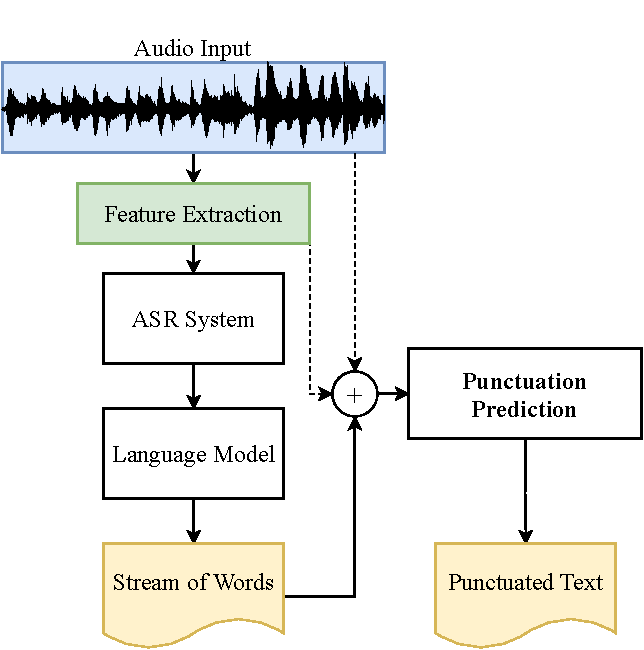
\includegraphics[width=0.50\textwidth]{1_1_01.pdf}
\caption{Punctuation in an ASR pipeline.}
\label{fig:1_1_01}
\end{figure}



 Creating a punctuation annotation system for this streamed case comes with the following challenges:
\begin{enumerate}
    \item When predicting punctuation immediately following each word, words appearing to the right of the possible punctuation mark are not available to the system. We call this \emph{lack of right-side context}.
    \item Using acoustic features as shown in Figure~\ref{fig:1_1_01}\Ondrej{Use Figure not figure} is likely to be more difficult in a streaming scenario, as information form\Ondrej{from} multiple parts of the pipeline has to be streamed to the punctuation prediction model. We call this \emph{reduced availability of acoustic features}.
    \item When predicting punctuation following every streamed word, we should, on average, not use more time than the average time that passes between two words\Ondrej{maybe ``average word duration'' would be better}. This is one of the most wanted characteristics, which we call the \emph{need for speed} of inference.
\end{enumerate}
While we reason that most existing punctuation annotation systems could be adapted to the lack of right-side context, the reduced availability of acoustic features could be hard to overcome in real-world applications. For example, if an ASR system provided as a service by a third party is used in an application, the recorded audio would, in addition to being sent to said ASR system, have to be stored locally and then aligned to the output produced by the ASR system for use with a punctuation annotation system.

\Ondrej{Summarise aims and contributions here}

\chapter{Background}

We now outline the methods used for punctuation annotation in the past, in the context of the streamed punctuation annotation task\Ondrej{remove the rest of the sentence} we have set out to solve.

\section{Existing Approaches to Punctuation Annotation}
Punctuation annotation using learned and statistical models has been studied for more than two decades, with the related task of sentence segmentation predating those efforts even further. We examine the different approaches to punctuation annotation in the following three sections:
\begin{enumerate}
    \item We examine the data used to train such systems, and how feature engineering has been used to get the most out of said data.
    \item We examine the learning methods used over time, and explain the recent rise of Transformer-based techniques.
    \item We give an overview and interpretation of previous results in terms of f1-scores on different punctuation marks, datasets and learning techniques.
\end{enumerate}

\subsection{Punctuation Data \& Feature Engineering}
\label{sec:features}

Early systems in the sentence segmentation and punctuation annotation domain \citep{palmer1995satz, beeferman1998} made use of datasets of written or read rather than spoken language, such as the Wall Street Journal corpus \citep{wsj} or Brown corpus \citep{browncorpus}. N-grams were successfully used by these early systems \citep{beeferman1998}, while auxiliary features such as POS tags were shown to improve performance as well \citep{palmer1995satz}. While earlier work founds commas to be easier to predict than full-stops as they require less lexical context \citep{beeferman1998}, it was later found that in the HUB-4 Broadcast News Corpus (BN) \citep{hub4}, commas are harder to predict than full-stops, in part due to weak human agreement on the correct placement of commas \citep{christensen2001,batista2008}. Experiments with features derived from acoustic data showed a significant improvement in predicting full stops when using pause durations and a modest improvement when including phone durations or pitch \citep{christensen2001}. Recent efforts in feature extraction use pretrained word and speech vectors to great effect \citep{che2016,zelasko2018,yi2019speech2vec}, but other works indicate there is a trade-off between the wider availability of text than speech features and the expressivity of speech features, leading to purely lexical models outperforming acoustic ones in certain settings due to more available training data \citep{Klejch2017}. With the rise of multi-task learning \citep{crawshaw2020multitask}, \Ondrej{part-of-speech} POS tags have seen renewed use \citep{yi2020adversarial}, but not as an additional input feature but as an additional model output. By training on both tasks, the model improves on the punctuation annotation task by benefiting from the information learned for the POS tagging task. The same principle has been applied using disfluency detection as well \citep{chen2020controllable}. 
Most recent work focuses on predicting full stop, comma and question punctuation marks, which we assume is motivated by their distinct functions in language. Less common punctuation marks contained in datasets are either discarded \citep{zelasko2018} or mapped to one of the common three classes. These punctuation marks include exclamation mark, paranthesis, dash, colon, semicolon and three dots and their mapping to one of the three punctuation classes most widely used is sometimes ambiguous, as for example three dots could be either mapped to comma or full stop \citep{gravano2009}.

\begin{table}[h]
\begin{center}
\begin{sc}
\begin{tabular}{|l|l|lll|}
\hline
\textbf{Dataset} & \textbf{Tokens} & \textbf{Full Stop} & \textbf{Comma} & \textbf{Question Mark} \\ \hline
WSJ              & 51,023          & 4.59\%             & 5.98\%         & 0.04\%                 \\
BN               & 35,710          & 3.5\%              & 5.1\%          & 0.29\%                 \\
IWSLT11              & 17,207          & 5.37\%             & 6.36\%         & 0.48\%                 \\
MGB              & 92,622          & 7.63\%             & 4.77\%         & 1.67\%                 \\ \hline
\end{tabular}
\end{sc}
\end{center}
\caption{Distribution of the three most commonly reported punctuation marks across the most widely used corporas' validation sets as reported by previous work.}
% \citep{kim2003,batista2008,Ueffing2013,Klejch2016}
\label{dspunc}
\end{table}
More recent work also focuses on newer datasets, with the most common one being the IWSLT2011 dataset \citep{iwslt2011}\Ondrej{I would write IWSLT~2011 and IWSLT~11 or just IWSLT}, which consists of IWSLT11\footnote{https://www.ted.com} talk transcripts. IWSLT11 talks, while delivered in a spoken form, are scripted in advance and rehearsed and are monologues rather than conversations. The MGB dataset, which consists of a wide range of TV broadcasts, has also been used, and contains more spontaneous speech and dialogues \citep{Bell2015}. The WSJ and BN datasets used in the past contain written and spoken news, respectively. The distribution of punctuation marks across datasets is shown in Table~\ref{dspunc} \Ondrej{Use Table~\ref{dspunc} with non-breaking space}.
The spoken nature of BN could explain the slight increase in question marks over WSJ. The IWSLT11 and MGB corpora are more informal and span more genres, which could explain the more common occurrence of question marks and full stops. Human annotators do not always agree on punctuation \citep{batista2008,interannotator2020}, which could also play a role in these differences. In related work, all of these datasets are processed in a similar fashion. First, the text is converted to a single, unsegmented transcript to avoid giving the model segmentation information that would not be present at inference time \citep{che2016}. Second, punctuation data is removed from the input ($X$) while the desired output ($y$) contains the removed punctuation. There are different ways to model $y$, and they are explained in detail in section \ref{sec:model} \Ondrej{Use Section~\ref{sec:model}}.
\begin{figure}[H]
\centering
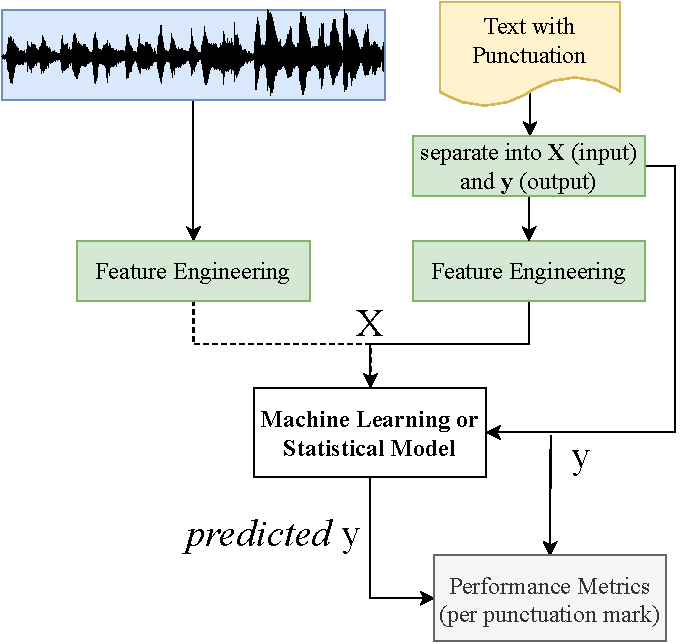
\includegraphics[width=0.50\textwidth]{2_1_1.pdf}
\caption{Punctuation annotation is learned using punctuated texts which are split into $X$ (no punctuation) and $y$ (punctuation target).}
\label{fig:learn}
\end{figure}
While we have now covered feature engineering and how the initial text is processed for punctuation annotation, we explain the learning methods that aim to utilize these datasets and features in the next section.

\subsection{Learning Methods}
\label{sec:learning}

Early neural-network-based approaches on the sentence segmentation task showed promising results \citep{palmer1995satz}, but early systems recovering punctuation models relied mostly on statistical language models such as Hidden Markov Models (HMMs) \citep{beeferman1998,Chen1999,christensen2001,briscoe2002}. These models did not perform well at modeling long-range dependencies required for end-of-sentence punctuation marks such as question mark or full stop \citep{beeferman1998}\Ondrej{because of Markov property?}. Their purely statistical nature also made it difficult to perform well on unseen sequences, even if they were semantically similar to sequences the model was trained on. A maximum entropy approach showed promising results as well \citep{Huang2002}.
Dynamic conditional random fields (CRFs) improved further on HMMs, and performed better at capturing said long-range dependencies \citep{LuNg2010,wangngsim2012}.  Further work explored deep neural networks in the form of Long short-term memory neural networks (LSTMs) \citep{Tilk2015,Klejch2017}. Experiments on knowledge distillation showed that a student model can leverage information from a teacher ensemble in the punctuation annotation domain \citep{yitaowen2017}. Recent work has shown promising results using attention-based models \citep{yi2019speech2vec,sunkara2020}. While pre-trained Transformer models such as BERT \citep{devlin2018} often performed better than models trained from scratch, recent work has introduced novel ways to combine lexical and acoustic features without forced alignment, such as sub-word attention models \citep{sunkara2020}. It has also been shown that jointly predicting POS tags and punctuation leads to improvements \citep{yi2020adversarial}.
Next, we contrast and compare recent work with respect to different punctuation marks, datasets, input features and learning methods.

\subsection{Evaluating Punctuation Prediction Models}
\label{sec:eval}
While the most frequently used evaluation metric for punctuation annotation is the $F_1$ score, the slot error rate (SER) can be used as well. As it is more common to report $F_1$ score on a per-punctuation mark basis, we use the $F_1$ scores reported by previous work in this section. Due to the majority class being \emph{no punctuation}, the recall and precision scores for punctuation annotation are computed over punctuation marks only: $$\text{precision}=\frac{\text{\# of correctly predicted punctuation marks}}{\text{\# of predicted punctuation marks}}$$

$$\text{recall}=\frac{\text{\# of correctly predicted punctuation marks}}{\text{\# of punctuation marks in reference}}$$

Using these recall and precision values, we can then compute the $F_1$ score as usual. For the remainder of this work, we report $F_1$ scores computed this way.

$$F_1 = \frac{2*\text{recall}*\text{precision}}{\text{recall}+\text{precision}}$$

\subsection{Overview of Punctuation Annotation}
\begin{figure}
\centering
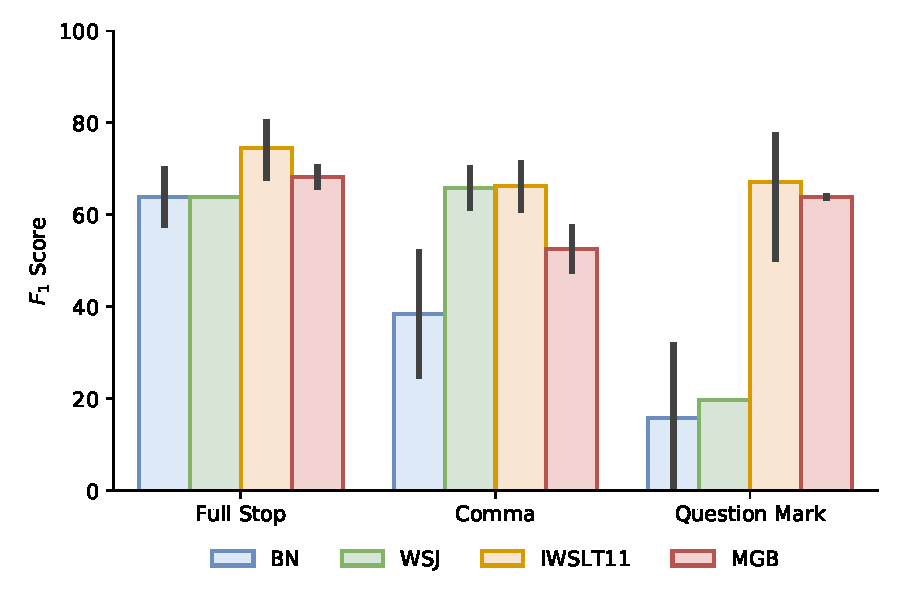
\includegraphics[width=.8\textwidth]{dataset_punctuation_new(1).pdf}
\caption{The  average $F_1$ scores achieved in previous work per dataset.}
\label{fig:datasetf1}
\end{figure}

As can be seen in Figure~\ref{fig:datasetf1}, periods are the only punctuation marks with similar scores across datasets. We attribute this to the combination of their relatively high occurrence (see Table~\ref{dspunc}) and little ambiguity. Question marks get very low scores in the BN and WSJ corpora which were used with purely statistical methods which made it difficult to capture the long-range dependencies needed to distinguish question marks from periods \citep{christensen2001,gravano2009}. Commas seem to be easier to recover on the WSJ corpus than the BN one, which we attribute to the spoken nature of the BN corpus. In general the lower scores on BN and WSJ as opposed to IWSLT11 and MGB should not be attributed to the datasets being more difficult, but rather shows the weaknesses of the purely statistical models used on these earlier datasets. The results on the IWSLT11 and MGB corpus are more indicative of modern deep-learning-based techniques, and show an important trend: the spoken nature of both the IWSLT11 and MGB corpus make commas the hardest symbols to predict, while question marks, although much less common, are close to periods in score. Previous work has shown that commas are the most ambiguous punctuation mark, with this ambigouity increases\Ondrej{grammar?} when utterances are unscripted \citep{interannotator2020}. Intuitively, the MGB corpus should lead to lower scores overall due to its more spontaneous and unscripted nature, and the data seems \Ondrej{to} confirm this. However, we caution to draw this conclusion, as state-of-the-art Transformer models have been used on the IWSLT11 dataset but not on the MGB dataset.

\begin{figure}
\centering
\begin{subfigure}{.49\textwidth}
\centering
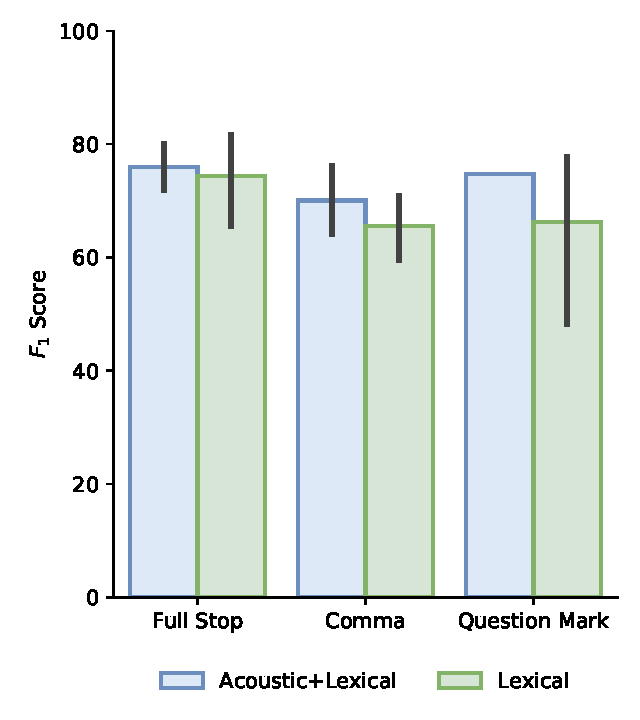
\includegraphics[width=.95\textwidth]{dataset_acoustic_lexical.pdf}
\caption{comparison of acoustic \& lexical features}%F-measures achieved in previous work per punctuation mark and dataset.}
\end{subfigure}
\begin{subfigure}{.49\textwidth}
\centering
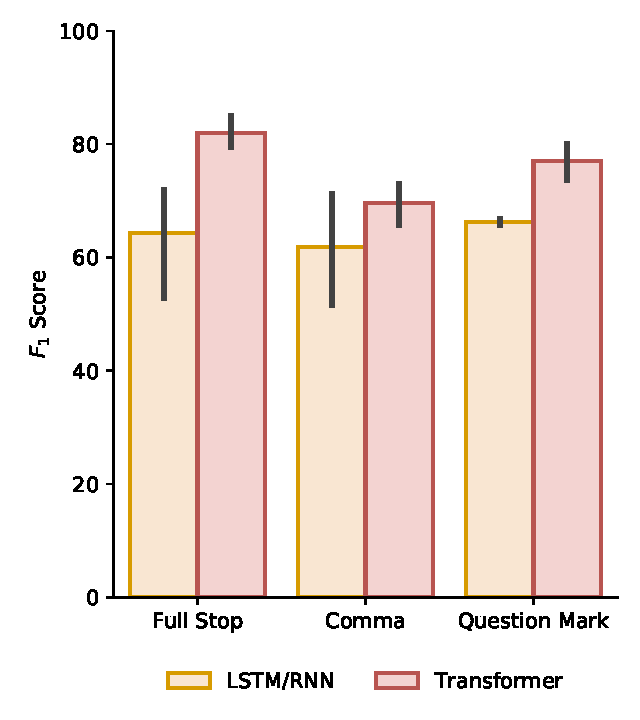
\includegraphics[width=.95\textwidth]{dataset_transformer.pdf}
\caption{comparison of LSTM/RNN \& Transformers}%F-measures achieved in previous work per punctuation mark and model architecture (on the IWSLT11 dataset).}
\end{subfigure}
\caption{The average $F_1$ scores achieved on the IWSLT11 dataset reference transcriptions, grouped by input features and model architectures.}
\end{figure}

As these differences between datasets are quite significant, and most recent work makes use of the IWSLT11 dataset, we conduct a more detailed analysis solely on papers predicting punctuation in the reference transcripts of the IWSLT11 dataset. While pre-training and additional data used varies across these works, this still allows insight into some general trends. First, we group models by their use of solely lexical or acoustic and lexical information, which reveals that models incorporating acoustic information generally perform better than ones without. The aforementioned drawback of less available training data when using acoustic information does not apply to one of these models however, as \citet{yi2019speech2vec} combine a pre-trained word embedding with pre-trained speech embeddings. This acoustic information comes in different forms as well: \citet{Tilk2015} use pause durations alone, while \citet{yi2019speech2vec} use Speech2Vec \citep{chung2018} to encode the original acoustic information into a vector. When comparing recurrent architectures such as LSTM or RNN with Transformers, a very clear trend emerges which shows Transformers to clearly outperform recurrent models on every punctuation mark except the comma. It is possible that Transformers outclass RNNs when it comes to long-range dependencies as the maximum path lengths between any two inputs is $\mathbf{O}(1)$ rather than $\mathbf{O}(n)$ due to self-attention \citep{vaswani2017}. Others\Ondrej{Other} reasons could be the availability of pre-trained Transformer models for NLP and their scalability, allowing for deeper models \citep{transformersurvey}. Comma prediction depends less on long-range context than end-of-sentence punctuation marks \citep{beeferman1998}, which we hypothesise explains the similarity of recurrent and Transformer architectures in this case. Overall, Transformers are state-of-the-art performers in the punctuation domain, and their architecture and functionality is explained next.


\section{Pre-trained Transformer Models in NLP}
Transformers, which achieve state-of-the-art performance in most tasks in the NLP domain, scale well with training data and model size \citep{huggingface}. In this section, we briefly outline the transformer architecture and how and why transformers are pre-trained using masked language modeling (MLM) and fine-tuned for sequence tagging and classification, and possible ways to speed up these models at inference time and reduce their size.\Ondrej{split into multiple sentences to simplify}

\subsection{Architecture of a Transformer Encoder}
\label{fig:transformerarch}
\begin{figure}
\centering
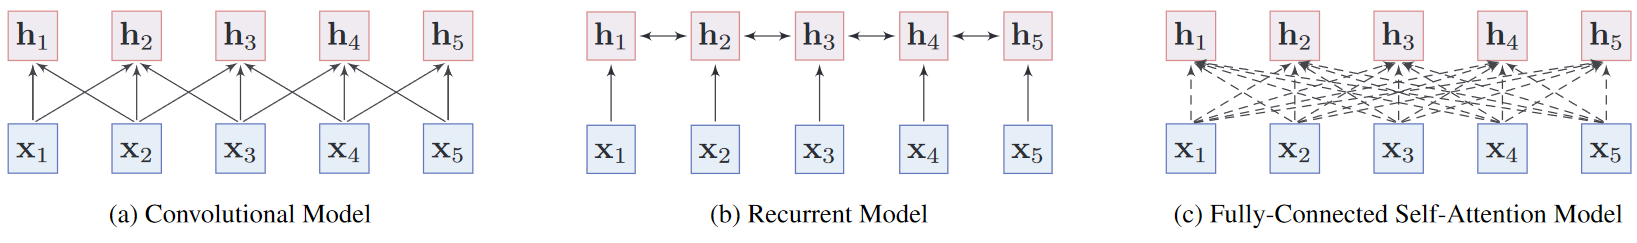
\includegraphics[width=\textwidth]{conv_rec_att.PNG}
\caption{Comparison of neural contextual encoders by \citet{transformersurvey}.}
\label{fig:attentioncomparison}
\end{figure}
\begin{figure}[H]
\centering
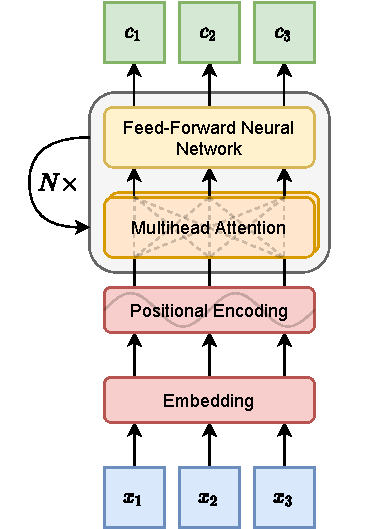
\includegraphics[width=.4\textwidth]{transformer(2).pdf}
\caption{Architecture of a Transformer Encoder}
\label{fig:transformerencoder}
\end{figure}
The central concept of Transformers is self-attention. As shown in Figure~\ref{fig:attentioncomparison} \citep{transformersurvey}, this self-attention allows a model to take all elements of the sequence into account, while also processing them at the same time. A Transformer encoder transforms a sequence of input tokens $x_i$ to contextualized word embeddings $c_i$ using the following steps \citep{vaswani2017}.
\begin{enumerate}
    \item Create a $d$-dimensional embedding for each input token. 
    \item As the transformer architecture processes all inputs simultaneously, position information is not inherently available to the model. To circumvent this, the $\sin$ and $\cos$ functions are used to generate values which differ at each input position, which are then added to each embedding based on its position. These slight variations in value based on position allow the transformer to learn from positional information without processing inputs in sequence.
    \item In a process called Self-Attention, create a key, value and query vector from each input, and transform each using a learned weight matrix. For each input, create one output $o_i$ as the weighed sum of all values based on the key and value dot product as follows: $$o_i=\sum_{j=1}^N \frac{\softmax(k_j\cdot q_i)}{\sqrt{d}}\times v_j$$ Note that it has been found that normalizing the weighed sum by dividing by $\sqrt{d}$ leads to more sTable~training \citep{vaswani2017}. When this process is repeated multiple times with independent weight matrices, we speak of Multihead Attention. The outputs of these multiple heads are concatenated in this case.
    \item A residual\Ondrej{might not be clear what residual is} is added to said output to avoid vanishing gradient, and the vector is passed through a feed-forward neural network. As can be seen in Figure~\ref{fig:transformerencoder}, this process can be repeated $N$ times, with popular architectures ranging between 6 and 24 of these blocks \citep{transformersurvey}.
    \item The resulting context vectors $c_i$ can be passed to a decoder for sequence-to-sequence tasks, or to a so-called \emph{head} for tasks with fixed-length target values, such as classification, tagging or regression.
\end{enumerate}
Next, we explain how the encoder is used in tandem with these heads to create pre-trained Transformer models for NLP.
%The most central concept of Transformers is self-attention, which transforms each element of a sequence into a weighed sum of all elements of said sequence, based on their dot-product similarity. To allow for positional information to be used, a positional encoding is added to each input. As shown in Figure~\ref{fig:attentioncomparison} \citep{transformersurvey}, this approach allows a model to take all elements of the sequence into account, while also processing them at the same time. In contrast, convolutional models can process elements at the same time but can only take a limited window of context into account, while recurrent models can model the whole context, but need to process elements one at a time, in sequence.

\subsection{Large, Pre-trained Models}
\label{sec:pretrained}
The lack of large amounts of task-specific, annotated data has lead to the rise in a range of pre-trained Transformer models. These models are trained using a range of pre-training objectives on large, unlabeled text datasets \citep{transformersurvey}. One of the most successful and widely-used models is BERT \citep{devlin2018}. BERT is pre-trained using masked token prediction, which randomly selects tokens in the input sequence and replaces them with a \texttt{[MASK]} token. The model then has to predict the original tokens at each masked position. A second task which used for pre-training BERT is next sentence prediction (NSP), in which the model has to solve the binary classification task of predicting if one sentence is followed by another. The goal is not to excel at these two tasks, but to train a model which produces hidden representations which can be used well for a variety of down-stream tasks. A variant of BERT called RoBERTa \citep{roberta} showed improved performance by computing the mask positions for MLM anew for each epoch rather than once before training. They also remove the NSP task and improving \Ondrej{grammar} batch size and other hyper-parameters. RoBERTa outperforms BERT on a diverse set downstream tasks \citep{roberta}. Another approach instead replaces a percentage of tokens with similar ones and train \Ondrej{trains?} the model as a discriminator \citep{electra}. Whichever set of pre-training tasks is chosen, their aim is to train a model which produces a contextualized embedding for each input token which can be used in downstream tasks. These embeddings could be used in a separate model, in the same way as \Ondrej{typically used word embeddings} GloVe \citep{pennington2014glove} or Word2Vec \citep{mikolov2013word2vec}. However, usually the whole model is adapted to a new task in a process called fine-tuning.

\begin{figure}
\centering
\begin{subfigure}{0.49\textwidth}
\centering
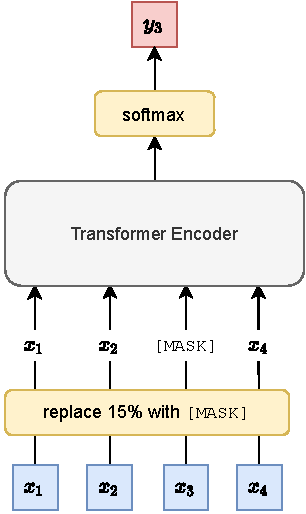
\includegraphics[height=.9\textwidth]{MLM(2).pdf}
\caption{Masked Language Modeling}
\label{fig:mlm}
\end{subfigure}
\begin{subfigure}{0.49\textwidth}
\centering
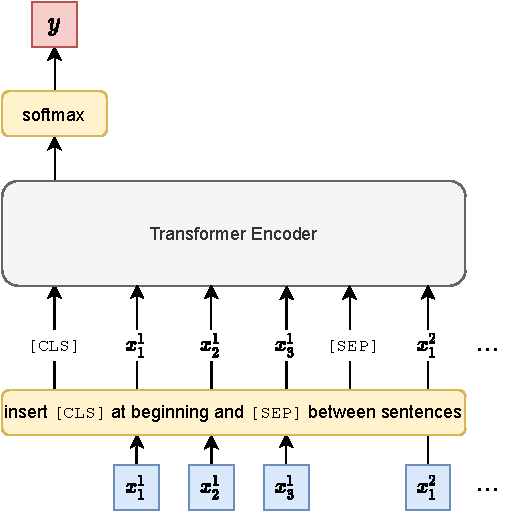
\includegraphics[height=.9\textwidth]{NSP.pdf}
\caption{Next Sentence Prediction}
\label{fig:mlm}
\end{subfigure}
\caption{The two pre-training tasks used in BERT.}
\end{figure}


\subsection{Fine-tuning for Punctuation Annotation}
\label{sec:finetuning}
When adapting a pre-trained Transformer to a downstream task, a task-specific \emph{head} is added after the Transformer encoder. Training the architecture with this task-specific head can yield good results even when training on few training samples \citep{huggingface}. Different tasks require different heads, but for punctuation annotation, the majority of previous work use either one or two linear layers \citep{chen2020controllable,sotapunctuation} or a bi-directional Long Short-Term Memory (Bi-LSTM) \citep{yi2020adversarial}. Conditional Random Fields (CRFs) in conjunction with RoBERTa were found to not improve performance by \citet{sotapunctuation}. It is also possible to add a decoder component and treat the problem as a sequence to sequence task \citep{yi2019speech2vec}.

\subsection{Inference Speed and Model Size}
\label{sec:speed}
A drawback of the transformer architecture is that the runtime and memory requirements of dot-product attention scales quadratically with sequence length ($\mathcal{O}(n^2)$) \citep{tay2020efficient}. A range of replacements of this expensive operation have been proposed such as Reformer \citep{kitaev2020reformer} and Linformer \citep{wang2020linformer}, which reduce this to $\mathcal{O}(n\log{}n)$ and $\mathcal{O}(n)$, respectively. However, to the best of our knowledge, no large-scale pre-trained models using these architectures are publicly available at the time of writing, negating the benefit of pre-trained Transformer models. Another way to improve inference speeds is to reduce the length of the input, which we explore in section \ref{sec:trunc}.\\ State-of-the-art punctuation annotation models rely on large Transformer models which are large in size. The best results achieved on the IWSLT11 dataset reference transcriptions we are aware of make use of \textsc{RoBERTa-large} \citep{sotapunctuation}, which has 355M parameters. When each weight is of type \texttt{float32}, this leads to a model size of 1.4GB. Recent work has shown that during training, Transformers benefit from this large number of weights and converge faster than when using smaller models \citep{li2020train}. \citet{li2020train} therefore suggest to train large Transformer models first, and to then quantize and/or prune the model weights. By compressing a model this way and then re-training on a subset of the original data, model size can be reduced to a fraction of its original size, while maintaining comparable performance \citep{han2016compression}. To the best of our knowledge, this has not been explored in the punctuation annotation domain.

\section{Ways to Model Punctuation Annotation}
\label{sec:model}
\begin{figure}
\centering
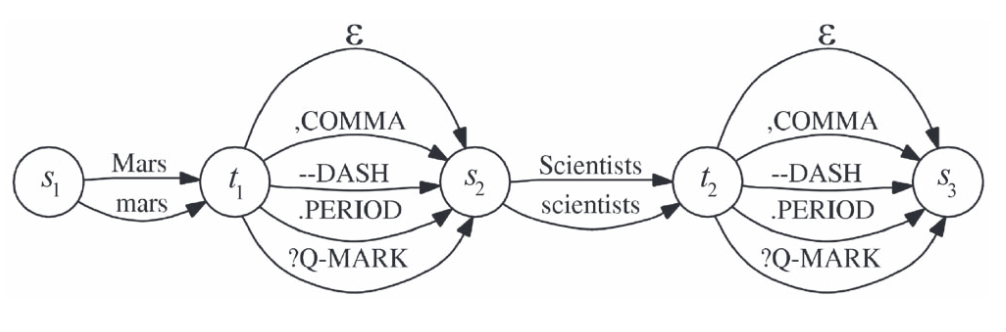
\includegraphics[width=0.8\textwidth]{gravanofst.PNG}
\caption{Punctuation- and capitalization-recovering finite-state machine by \citet{gravano2009}.}
\end{figure}

As discussed in section \ref{sec:learning}, early punctuation annotation systems mainly use statistical methods, such as Finite-state Machines (FSMs) in conjunction with Viterbi Decoding, to recover punctuation. These approaches found valuable information still useful today such as the strong predictive power of pause durations \citep{christensen2001} and the limited context required for predicting comma \citep{beeferman1998}, but the statistical models themselves were replaced by a variety of neural network architectures. Until recently, the main contenders among these were recurrent \citep{Tilk2015,Klejch2016,yitaowen2017}, and less frequently, convolutional \citep{che2016} neural networks. In recent years, the trend of the Transformer architecture achieving state-of-the-art results in many NLP domains \citep{transformersurvey} has extended to punctuation annotation as well \citep{yi2019speech2vec,chen2020controllable,sotapunctuation}. While statistical models model punctuation as a probability distribution over possible events occurring between words, there are three other ways to model punctuation annotation which have emerged alongside learning-based models in NLP:

\begin{figure*}[h]
\centering
\begin{subfigure}{.3\textwidth}
\centering
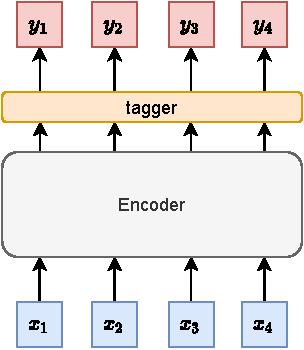
\includegraphics[width=.95\textwidth]{tagging.pdf}
\caption{}
\end{subfigure}
\begin{subfigure}{.3\textwidth}
\centering
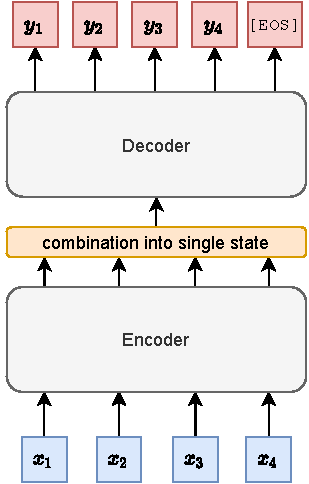
\includegraphics[width=.95\textwidth]{translation.pdf}
\caption{}
\end{subfigure}
\begin{subfigure}{.3\textwidth}
\centering
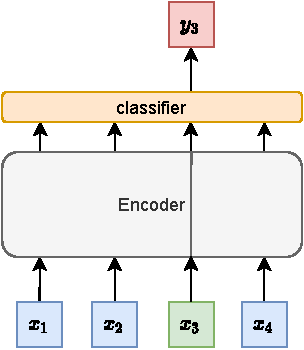
\includegraphics[width=.95\textwidth]{classification(2).pdf}
\caption{}
\end{subfigure}
\centering
\caption{Three possible ways to model punctuation using neural network encoders are (a) tagging each element based on its contextualized embedding, (b) treating the task as a translation problem and creating punctuation using a decoder (c) classifying a single element in the input sequence. \Ondrej{Is the arrow over encoder in (c) intentional?}}
\end{figure*}

\begin{enumerate}[label=(\alph*)]
    \item \emph{Tagging:} For models which create one state for each element in the input sequence, such as recurrent neural networks (RNNs) or Transformers, a final tagging layer can predict the punctuation mark associated with each such element. When using this approach with the Transformer architecture, punctuation marks predicted earlier in the sequence cannot be used for later predictions. This limitation can be overcome by using an RNN as the tagging head as described in section \ref{sec:finetuning}. Some previous work successfully use Conditional Random Fields (CRFs) as well \citep{yi2020adversarial}, while the work reporting the best results on the IWSLT11 dataset as of the time of writing finds no improvement from CRFs \citep{sotapunctuation}.
    \item \emph{Machine Translation:} The hidden state(s) produced by a neural network encoder can also be fed to a decoder, which then outputs a sequence of punctuation marks. This approach can make use of previously predicted punctuation marks, but requires the model to learn to output the same number of marks as are words in the input.
    \item \emph{Classification:} A model can also be trained to predict one punctuation mark per input. The position of the punctuation mark can either be static or given to the model as an additional input. The drawback of this approach is that one inference step is required for each word in the input sequence.
\end{enumerate}

\begin{table}[H]
\begin{tabular}{ll}
\hline
\textbf{Approach}                   & \textbf{Paper} \\ \hline
\multicolumn{1}{l|}{Tagging}        &
\specialcell{\citet{Tilk2015,yitaowen2017,chen2020controllable}\\\citet{yi2020adversarial,sotapunctuation}}
\\
\multicolumn{1}{l|}{Machine Translation}             & \specialcell{\citet{Klejch2016,Klejch2017,yi2019speech2vec}}                 \\
\multicolumn{1}{l|}{Classification} & \specialcell{\citet{che2016}}                 \\ \hline
\end{tabular}
\caption{Differing approaches for modeling punctuation annotation in previous work.}
\label{tab:approaches}
\end{table}

All of the above have been successfully used for punctuation annotation, as can be seen in Table~\ref{tab:approaches}. While there are more examples for tagging and machine translation, to the best of our knowledge, \citet{che2016} present the only approach using classification. We reason that this is due to the increased resources required when doing inference for each word rather than being able to do inference on a full sequence. In the next section, we show how for \emph{streamed} punctuation annotation, this classification approach can be advantageous, and present the \emph{Streamed Classification Punctuation Transformer}.


\chapter{Streamed Classification Punctuation Transformer}
This chapter outlines a proposed architecture for predicting punctuation in a streamed setting, such as at last step of the ASR pipeline. The desiderata for this system are (1) ability to use in a streamed setting with limited lookahead (2) favourable performance compared to state-of-the-art (3) real-time inference speed.

\section{Masked Punctuation Prediction}
\label{sec:modelsetup}
\begin{figure}[!htbp]
\centering
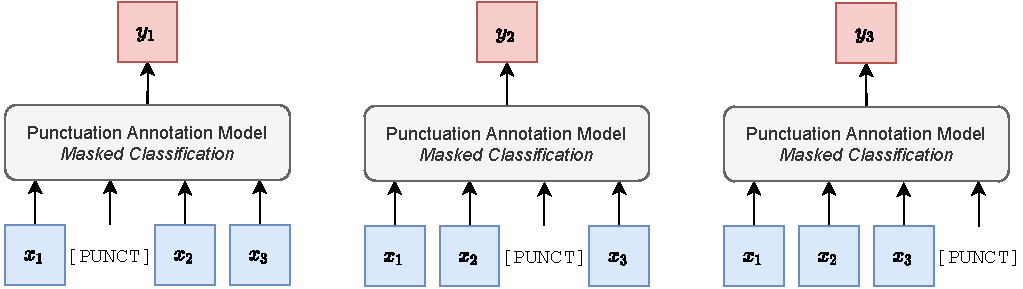
\includegraphics[width=\textwidth]{maskedpunct.pdf}
\caption{Punctuation annotation as a classification task using a \texttt{[PUNCT]} token.}
\label{fig:maskedpunct}
\end{figure}
In real-time settings, there is a \emph{lack of right-side context}: an ASR streams words to the punctuation system and punctuation is added continuously. The less right-side context a model needs, the earlier can a punctuation mark be inserted into the final output.
\begin{figure}[h]
\centering
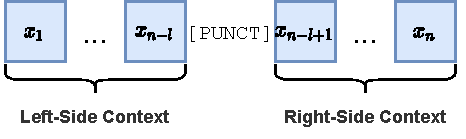
\includegraphics[width=.5\textwidth]{rightleft(1).pdf}
\caption{Left- and right-side context in masked punctuation prediction.}
\label{fig:rightleft}
\end{figure}
\begin{figure}[h]
\centering
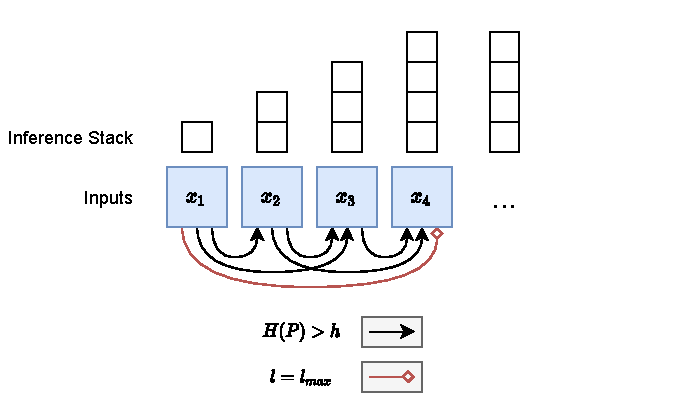
\includegraphics[width=0.8\textwidth]{inferencestack.pdf}
\caption{Inferences stack for $l_{max}=3$, assuming $H(P)>h$ at each time step.}
\label{fig:infstack}
\end{figure}
However, as discussed in section \ref{sec:model}, most recent punctuation annotation systems model the problem as a tagging or sequence-to-sequence task and use deep learning models. For these models, the training objective is loss minimization. When modeled as a tagging or sequence-to-sequence task however, this loss term includes equal parts of each output, regardless of its position within the sequence. We argue that a model facing little right-side context will perform better when trained exclusively on samples with little right-side context, and propose Masked Punctuation Prediction for this purpose. Inspired by the masked language modeling (MLM) and next sentence prediction (NSP) tasks used in pretraining \citep{roberta}, we insert a special \texttt{[PUNCT]} token into each training sample. The model is then tasked to predict the punctuation present at the location of this token using a classification head. As can be seen in Figure~\ref{fig:maskedpunct}, this requires one sample per punctuation mark. In a streamed setting, this is not a drawback however, as inference has to be run at the arrival of every new word in any case. When trained with a fixed-length right-side context, this token would not be necessary, as the model could learn the position of the punctuation over time. If we use varying lookahead however, this token is needed, as it encodes the punctuation position, and in turn the length of the current lookahead. Next, we describe this varying lookahead and how it can be used in practice.

\section{Varying Lookahead and Decoding}
\label{sec:entropyalgo}
\Ondrej{I feel like this section and section 3.1 could be expanded to provided better explanation. I am getting lost here and there.}

To predict punctuation in a streamed setting, we need a way to progressively feed the model more right-side context should it fail to predict punctuation with the context it is given initially, and make it robust to predicting sequences with varying lengths of this context. Using the \texttt{[PUNCT]} token described above, this can be achieved when training the model: We set the minimum and maximum lookahead ($l_{min}$ and $l_{max}$), and the \Ondrej{then?} insert the \texttt{[PUNCT]} token at $n-l$ for each sample, where $n$ is the sequence length and $l$ is the lookahead. The lookahead can by \Ondrej{be?} cycled through or drawn randomly from $[l_{min}, l_{max}]$.\\
For inference, a decoding strategy utilizing varying lookahead is needed, which we propose in Algorithm~\ref{alg:decoding}.
\begin{algorithm}
\SetAlgoLined
\KwData{$N$ = \texttt{List}(maxsize: $l_{max}+1$), $L$ = \texttt{List}}
\SetKwInOut{Input}{input}\SetKwInOut{Output}{output}
\Input{$token$, $h$}
\Output{$punctuations$, $positions$}
$punctuations \leftarrow $\texttt{List}, $positions \leftarrow $\texttt{List}

$L\leftarrow $ $L~\cup~token$

$P \leftarrow $ \textit{probabilities}($L$ $\cup$ \texttt{[PUNCT]})

\eIf{$H(P)>h$}{
    $N \leftarrow N \cup 0$
}{
    $punctuations \leftarrow punctuations \cup \text{argmax}(P)$
    
    $positions \leftarrow positions \cup 0$
}
\For{i $\leftarrow 1$ \KwTo $|N|$}{
    $n \leftarrow N_i$

    $P \leftarrow $ \textit{probabilities}($\{L_i\}_{i=0}^{|L|-n}$ $\cup$ \texttt{[PUNCT]} $\cup$ $\{L_i\}_{i=|L|-n+1}^{|L|}$)
    
    \eIf{$H(P)>h$}{
        $N_i \leftarrow n+1$
    }{
        $punctuations \leftarrow punctuations \cup \text{argmax}(P)$
        
        $positions \leftarrow positions \cup -n$
        
        $N \leftarrow N \setminus n$
    }
}
\caption{Entropy Threshold Decoding}
\label{alg:decoding}
\end{algorithm}
The first question that presents itself is how we decide if the system is predicting punctuation with reasonable confidence, or if more context is needed. We solve this by computing the Shannon-Entropy \citep{entropy} $H$ over the set of probabilities $p_i,...,p_k\in P$ assigned to each of the $k$ punctuation marks after the $\softmax$ step.
$$H(P)=H(p_i,...,p_k)=-\sum_{i=1}^k p_i \log_2 p_i$$
This value can be understood as the uncertainty of the model, and will be lower when the model is more certain of a prediction, being $0$ when one probability is $1$ and all others are $0$. Given the four possible outcomes of comma, period, question mark and no punctuation, the maximum value is reached when all probabilities are $\frac{1}{4}$ which corresponds with $H(P)=2$. For decoding, we set an entropy threshold $h$ and wait for more right-side context and repeat inference if the computed entropy $H(P)>h$. This is repeated until $H(P)\leq h$ or $l_{max}$ is reached. As words are streamed into the system, we potentially do inference on multiple punctuation positions at the same time step, with the maximum number of inferences conducted at the same time being $l_{max}+1$ as long as $l_{min}=0$, as can be seen in Figure~\ref{fig:infstack}.

\section{Adding Pause Tokens}
\label{sec:pausetok}

As described in section \ref{sec:features}, pause features have been shown to be strong indicators of punctuation \citep{christensen2001}. Given our setup of a pre-trained Transformer with a classification head (see section \ref{sec:modelsetup}), we see two ways to make these features available to the model:
\begin{enumerate}
    \item Concatenate pause durations following each word to the context vectors described in section \ref{fig:transformerarch} before passing them to the classification head.
    \item Add a \texttt{[PAUSE]} token after each word followed by a pause above a certain threshold.
\end{enumerate}
While 1) can include information on all pauses, rather than exclusively ones above a certain threshold, the only the classification head can learn from these features, while the Transformer encoder cannot. 2) on the other hand cannot encode all pause information, but enables the full architecture to learn from the pause features. For these reasons, our approach uses \texttt{[PAUSE]} tokens.

\begin{figure*}
\centering
\begin{subfigure}{.49\textwidth}
\centering
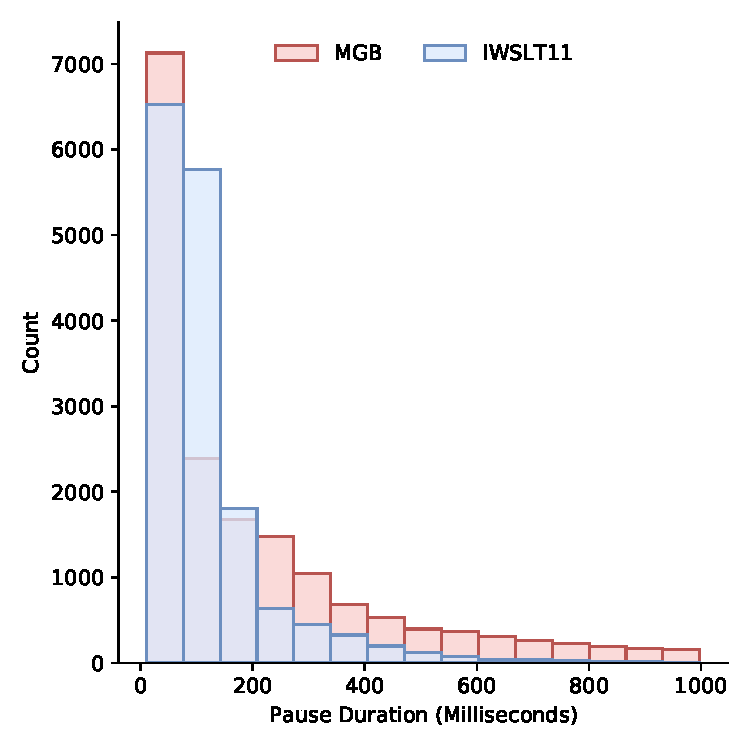
\includegraphics[height=.95\textwidth]{pausedist.pdf}
\caption{Distribution of pauses $\geq 10ms$}%F-measures achieved in previous work per punctuation mark and dataset.}
\end{subfigure}
\begin{subfigure}{.49\textwidth}
\centering
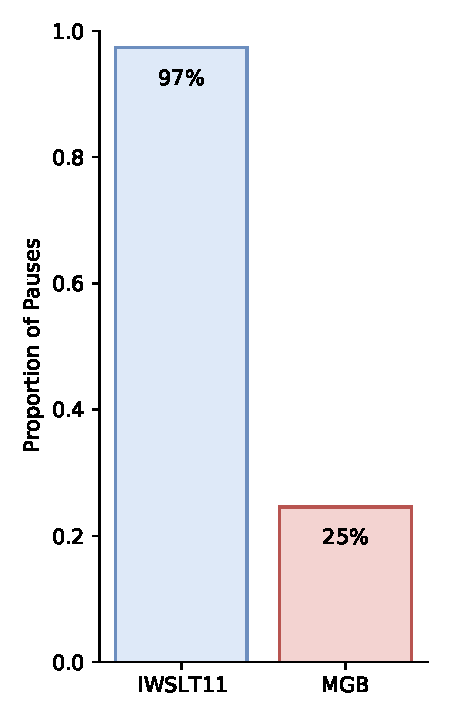
\includegraphics[height=.915\textwidth]{pauseprop.pdf}
\vspace{.2cm}
\caption{Word transitions with  pauses $\geq 10ms$}%F-measures achieved in previous work per punctuation mark and model architecture (on the IWSLT11 dataset).}
\end{subfigure}
\caption{Pause statistics of the MGB and IWSLT11 datasets.}
\label{fig:exppausedecay}
\end{figure*}

For a streamed punctuation system, pause durations can either be a part of the output of said system or can be approximated by measuring the time between words streamed. However for training, transcripts for both the IWSLT11 and MGB datasets do not contain timing information. On the other hand, ASR output for both systems including this information is available. Previous work aligns ASR outputs and transcripts to add punctuation to the ASR output \citep{yi2019speech2vec}. Inspired by this approach we first add \texttt{[PAUSE]} tokens to the ASR output using the available timing information, and then align this modified ASR output with the original transcripts using the \citet{needleman1970} algorithm. We publish our code to load the publicly available IWSLT11 dataset with and without pause durations\footnote{\url{https://github.com/MiniXC/punctuation-iwslt2011}}.
One drawback of this method is that for the IWSLT11 dataset, only the validation and test splits of the data come with ASR transcripts. To combat this we can a) use training data without pause durations first b) use MGB training data first and then finetune. For both approaches, we finetune the model using the validation set. a) and b) can also be used in combination as well. We evaluate these options empirically in section \ref{sec:pauseexp}. When using the MGB dataset for this purpose, it becomes worthwhile to investigate the pause duration similarity in both datasets. As can be seen in Figure~\ref{fig:exppausedecay}, both datasets follow a similar exponential decay when considering all pauses $\geq 10ms$, although the MGB dataset has a higher proportion of pauses in the range of $[0, 75]$ while the proportion of pauses in IWSLT11 is higher in the interval of $[75,150]$. We also observe a big discrepancy between the occurrence of pauses $\geq 10ms$, with 97\% of word transitions being accompanied by at least a short pause in the IWSLT11 dataset, while this is the case for just 25\% of transitions between words in the MGB dataset. We expect this to be the case due to the spontaneous vs. scripted nature of the MGB and IWSLT11 datasets (see section \ref{sec:features}). The dataset ASR transcriptions were possibly generated using differing systems, which could cause this difference as well. To combat this imbalance when training on one of the datasets and evaluating on the other, we can either take speaking rate into account or find the threshold that leads to the most similar statistics.
\begin{figure}
\centering
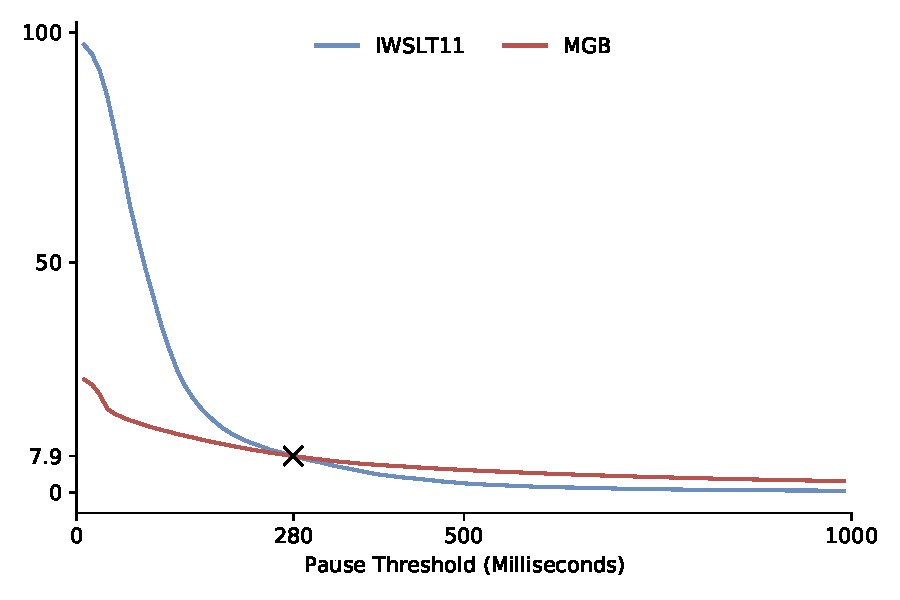
\includegraphics[width=.7\textwidth]{pause_threshold.pdf}
\caption{The proportion of pauses between words based on threshold $t_p$.}
\label{fig:idealthreshold}
\end{figure}
In this work, we use the latter approach and find that for $t_p\approx 280ms$, both datasets have a pause proportion of 7.9\%, as can be seen in Figure~\ref{fig:idealthreshold}. We evaluate this and other threshold values in section \ref{sec:pauseexp}. Next, we show how input truncation helps overall model efficency.

\section{Input Truncation for Faster Training and Inference}
\label{sec:window}
\begin{figure}[!htb]
\centering
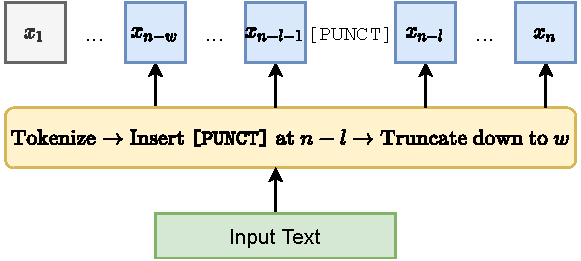
\includegraphics[width=.6\textwidth]{truncate.pdf}
\caption{Tokenization, \texttt{[PUNCT]} token insertion and truncation.}
\label{fig:idealthreshold}
\end{figure}
As described in section \ref{sec:speed}, Transformers use dot-product self-attention, which has a time and memory complexity of $\mathrm{O}(n^2)$. While there are architectures which reduce this to $\mathrm{O}(n\log n)$ or $\mathrm{O}(n)$, no large pre-trained models of such variants are available at the time of writing, negating the benefits we outline in section \ref{sec:pretrained}. As in many other punctuation annotation research \citep{Tilk2015,yi2019speech2vec,sotapunctuation}, we generate samples by using a sliding window on a transcript with all prior segmentation removed. Due to our approach of only predicting one punctuation mark at a time however, we are able to trim left-side context until we notice a degradation in performance. This is done after tokenization, as some Transformer architectures rely on a one-to-many mapping between words and embeddings. We introduce a parameter $w$ which determines the length of the window after truncation. We empirically evaluate different values of $w$ in terms of speedup and model prediction performance. Next, we discuss how we handle class imbalance in our punctuation annotation system.\Ondrej{I would remove this sentence}

\section{Punctuation Class Imbalance}
\begin{figure}[!htb]
\centering
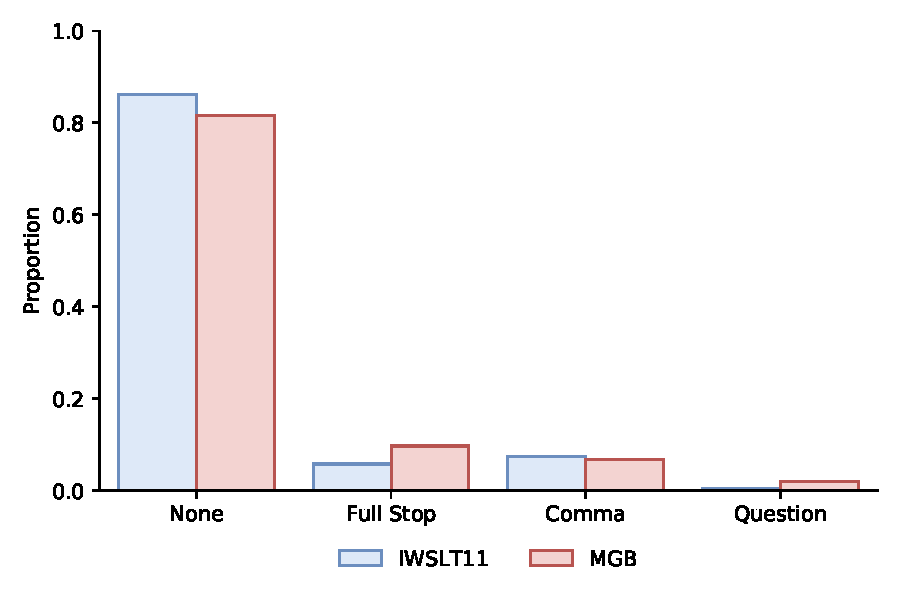
\includegraphics[width=.6\textwidth]{classimbalance.pdf}
\caption{Class distribution of the MGB and IWSLT11 validation datasets.}
\label{fig:classdist}
\end{figure}
When treating punctuation annotation as a classification problem, we encounter the class imbalance shown in Figure~\ref{fig:classdist}. Models trained on such datasets with imbalanced classes can develop a prediction bias for the majority class \citep{imbalance}. While there are many approaches for preventing this, \emph{under-sampling}, where part of the majority class data is discarded and \emph{over-sampling}, where part of the minority classes is repeated are the most common and robust ones \citep{imbalance}. When over-sampling, the repeated data can be augmented as well, by replacing words or characters in the input with similar ones \citep{ma2019nlpaug}. In this work, we rely on downsampling as a means to train large models efficiently. In the next chapter, we evaluate all techniques described in this chapter and present their best combination as our system.
\Ondrej{Move the last sentence into a new section called summary and summarise the whole chapter}


\chapter{Experiments and Results}
We now put our proposed architecture to the test and empirically evaluate how different methods affect performance on the MGB and IWSLT11 datasets. We make the scripts used for all experiments publicly available at \url{https://github.com/MiniXC/SAPAUT}.

\section{IWSLT11 and MGB Dataset \& Statistics}
\label{sec:notrain}
\begin{table}[h]
\begin{sc}
\begin{tabular}{@{}lllll@{}}
\toprule
\textbf{Dataset}                                & \textbf{Samples}               & \textbf{Full Stop} & \textbf{Comma} & \textbf{Question Mark} \\ \midrule
\multicolumn{1}{l|}{$\text{MGB}_{TRAIN}$}            & \multicolumn{1}{l|}{2.49M}          &   8.36\%                &         5.72\%       &    1.28\%                     \\
\multicolumn{1}{l|}{$\text{MGB}_{TRAIN \leftrightarrow ASR}$}     & \multicolumn{1}{l|}{2.04M}          &   8.43\%            &   5.83\%            &     1.25\%            \\
\multicolumn{1}{l|}{$\text{MGB}_{VALID}$}            & \multicolumn{1}{l|}{93,023}          &  9.74\%                  &       6.76\%         &          2.01\%              \\
\multicolumn{1}{l|}{$\text{MGB}_{VALID\leftrightarrow ASR}$}            & \multicolumn{1}{l|}{76,642} &       10.24\%             &   6.86\%             &         1.98\%               \\ \midrule
\multicolumn{1}{l|}{$\text{IWSLT11}_{TRAIN}$}        & \multicolumn{1}{l|}{2.4M}          &    6.13\%                 &        6.94\%        &      0.52\%                   \\
\multicolumn{1}{l|}{$\text{IWSLT11}_{VALID}$}        & \multicolumn{1}{l|}{49,279}          &  5.82\%                   &        7.46\%        &       0.54\%                 \\
\multicolumn{1}{l|}{$\text{IWSLT11}_{VALID\leftrightarrow ASR}$} & \multicolumn{1}{l|}{47,429}          &     6.27\%              &         7.50\%        &        0.54\%              \\
\multicolumn{1}{l|}{$\text{IWSLT11}_{TEST}$}         & \multicolumn{1}{l|}{14,312}          & 6.19\%                   &       5.79\%         &         0.35\%               \\
\multicolumn{1}{l|}{$\text{IWSLT11}_{TEST\leftrightarrow ASR}$}  & \multicolumn{1}{l|}{13,518}          &   6.73\%                 &      5.97\%          &     0.37\%                   \\ \bottomrule
\end{tabular}
\end{sc}
\caption{Statistics of the MGB and IWSLT dataset splits.}
\label{tab:datasetstat}
\end{table}
As can be seen in Table~\ref{tab:datasetstat}, the datasets splits aligned with the ASR transcripts (e.g. $TEST\leftrightarrow ASR$) are slightly smaller due to not all talks appearing in the transcripts. To allow for a fair comparison, we use the aligned splits for all experiments. The $\text{IWSLT11}_{TRAIN}$ dataset split does not come with ASR transcripts, and we can therefore only use it without pause information. \Ondrej{try to avoid having only a half a line on a new page}

\section{Pre-Trained Models by Huggingface}
The Huggingface Transformers library \citep{huggingface}, offers a range of pre-trained transformer models in conjunction with differing heads for finetuning. As described in section \ref{sec:finetuning}, based on the downstream task in question, a simple linear layer with $n_{classes}$ output nodes might be used for classification, while recurrent layers can be used for sequence tagging tasks.

\section{Baseline using Tagging Approach}
\begin{figure}
\centering
\begin{subfigure}{.49\textwidth}
\centering
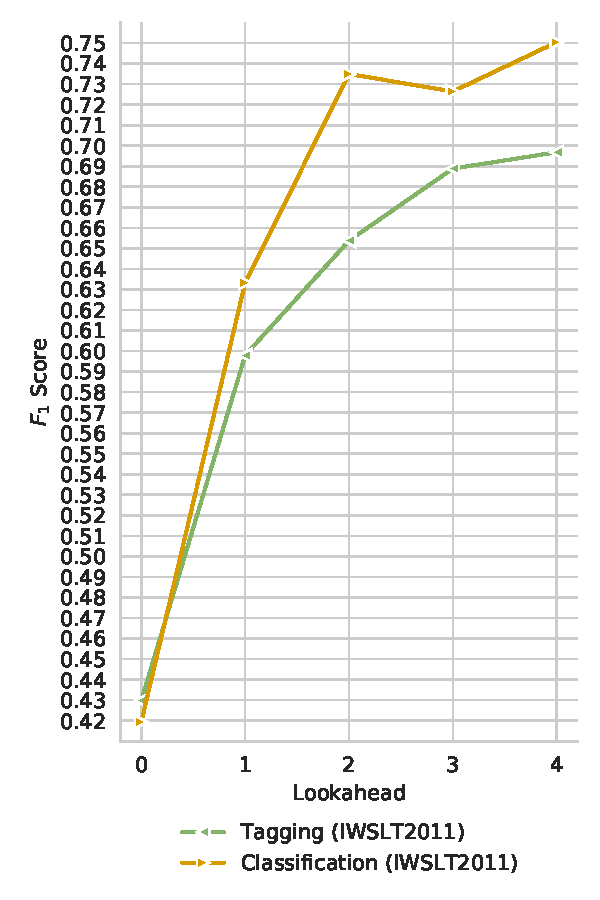
\includegraphics[width=.95\textwidth]{tagclassiwslt.pdf}
\caption{IWSLT2011 dataset}
\end{subfigure}
\begin{subfigure}{.49\textwidth}
\centering
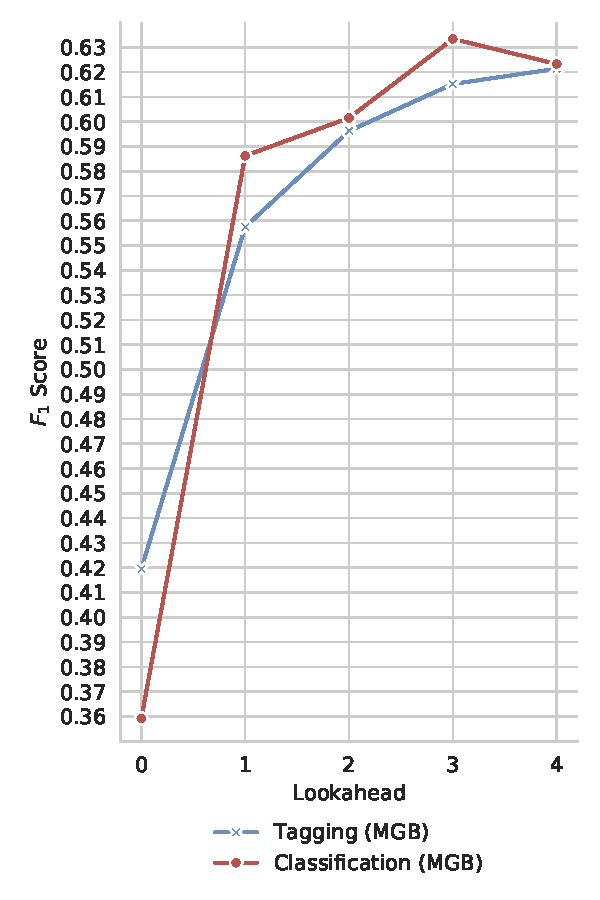
\includegraphics[width=.95\textwidth]{tagclassmgb.pdf}
\caption{MGB dataset}
\end{subfigure}
\caption{The $F_1$ scores achieved given different lookahead values.}
\label{fig:baselinelookahead}
\end{figure}
As our baseline to compare against, we train a model using the widespread sequence tagging approach \citep{Tilk2015,yitaowen2017,chen2020controllable,yi2020adversarial,sotapunctuation} with a Bi-LSTM head. The pre-trained model used is \textsc{DistilRoBERTa}, which is a \textsc{RoBERTa} variant \citep{roberta} distilled into a smaller model using the approach described by \citet{distilbert}. In preliminary experiments we find the hyper-parameters shown in Table~\ref{tab:hyped} to lead to robust results, and use said parameters for the remainder of experiments. We use the sliding window approach described in \ref{sec:window} with a window size of $w=32$ and evaluate using the $F_1$ measure described in section \ref{sec:eval} at different lookaheads. As can be seen in Figure~\ref{fig:baselinelookahead}, the classification model outperforms the tagging one for all lookaheads except $l=0$. We reason that this is due the classification model putting more emphasis on samples with little right-side context, as hypothesised in section \ref{sec:modelsetup}. The better performance of the tagging model on lookahead $l=0$ is surprising, but could be due to the tagging model having access to previous predictions using its Bi-LSTM layer, which the classification model has not. Preliminiary \Ondrej{Preliminary} experiments showed no significant improvements beyond a lookahead of 4. Therefore, to be able to compare to previous work, which has no limitations on right-side context, we evalute \Ondrej{evaluate} the per-class performance of models given a lookahead of 4 for this baseline (see Table~\ref{tab:baselineperclass}) and for the remainder of experiments. We notice that the classification approach yields a significant improvement for the IWSLT11 dataset, while not doing so on the MGB dataset.

\begin{table}[]
\centering
\begin{tabular}{ll}
\hline
\multicolumn{2}{c}{\textbf{Hyper-Parameters}}                               \\ \hline
\multicolumn{1}{l|}{Learning Rate (Initial/Maximum/Final)} & 1e-6/5e-5/1e-7 \\
\multicolumn{1}{l|}{Learning Rate Schedule}                & 1-cycle \citep{1cycle}        \\
\multicolumn{1}{l|}{Batch Size}                            & 128            \\
\multicolumn{1}{l|}{Optimizer}                          & AdamW \citep{adamw}           \\ 
\multicolumn{1}{l|}{Weight Decay}                          & 0.01           \\ \hline
\end{tabular}
\caption{Hyper-parameters used for all experiments.}
\label{tab:hyped}
\end{table}

\begin{table}[]
\begin{sc}
\resizebox{\textwidth}{!}{%
\begin{tabular}{@{}lrccc|ccc|ccc|ccc@{}}
\toprule
\multirow{2}{*}{Test}    & \multicolumn{1}{c}{\multirow{2}{*}{Model}} & \multicolumn{3}{c}{Full Stop}                    & \multicolumn{3}{c}{Comma}                        & \multicolumn{3}{c}{Question}                     & \multicolumn{3}{c}{Overall}                      \\ \cmidrule(l){3-14}
                         & \multicolumn{1}{l}{}                       & P              & R              & $F_1$       & P              & R              & $F_1$       & P              & R              & $F_1$       & P              & R              & $F_1$      \\ \midrule
\multirow{2}{*}{IWSLT11} & Tagging                    & \textbf{75.0} & 78.6          & \textbf{76.7}          & 58.8          & \textbf{64.7}          & 61.6          & \textbf{76.9} & 78.9          & \textbf{77.9} & 67.3          & 72.1          & 69.6          \\
                         & Class.             & 74.5          & \textbf{84.9} & 79.4 & \textbf{69.1} & 71.5 & \textbf{70.1} & 50.0          & \textbf{80.0} & 61.5          & \textbf{71.6} & \textbf{78.7} & \textbf{75.0} \\ \midrule
\multirow{2}{*}{MGB}     & Tagging                    & \textbf{65.4} & 68.6          & 67.0          & 56.1          & \textbf{52.9} & \textbf{54.5} & 62.4          & \textbf{62.4} & \textbf{62.4} & 61.8          & \textbf{62.1} & 62.0          \\
                         & Class.             & 63.4          & \textbf{72.0} & \textbf{67.4} & \textbf{59.9} & 48.8          & 53.8          & \textbf{71.0} & 55.3          & 62.2          & \textbf{63.0} &            61.6    & \textbf{62.3} \\ \bottomrule
\end{tabular}%
}
\end{sc}
\caption{Tagging and classification results for lookahead $l=4$.}
\label{tab:baselineperclass}
\end{table}

\section{Truncation Window Sizes}
\label{sec:trunc}

\begin{figure}[t]
\centering
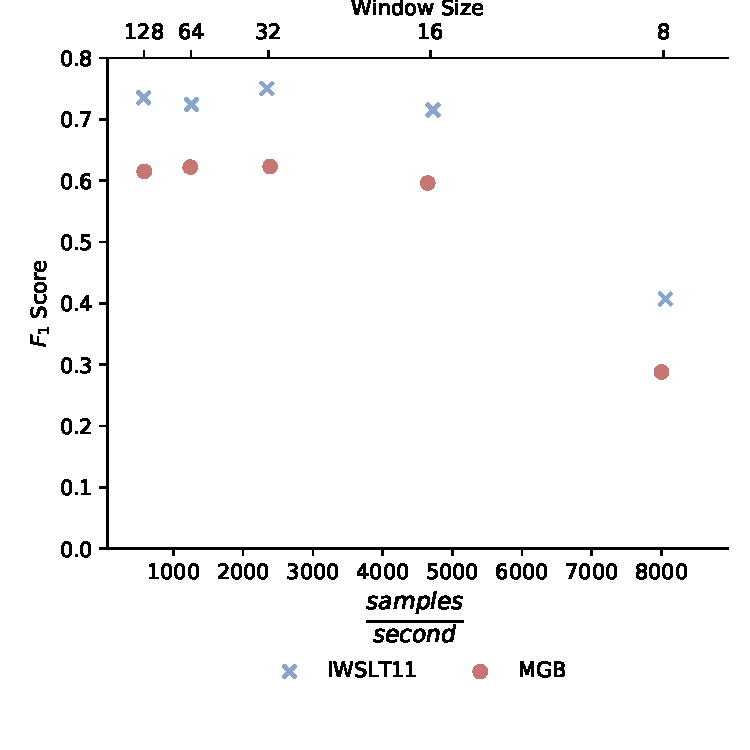
\includegraphics[width=.7\textwidth]{winsize(1).pdf}
\caption{Window size effect on speed and performance.}
\label{fig:winsize}
\end{figure}


So far, we have mainly focused on \emph{right-side context}, as it is a major limiting factor for streamed punctuation prediction. \emph{Left-side context}, on the other hand, can be limited on purpose to speed up training and inference. Due to the $\mathrm{O}(n^2)$ complexity of dot-product attention (see section \ref{sec:model}), every halving of the input should result in a quadratic reduction in inference and training time. We therefore truncate the left side of the input as described in section \ref{sec:window} and compare window sizes $w$ of 128, 64, 32, 16 and 8. Instead of the theoretically possible $\times4$ speedup for each halving we observe a $\approx\times2$ increase in speed. There also seem to \Ondrej{seems to be} diminishing returns, as the decrease from 16 to 8 in window size yields the lowest speedup in relative terms. As can be seen in Figure~\ref{fig:winsize}, decreasing the window size to below 32 decreases performance on both datasets. We therefore use a window size of 32 for all future experiments.

\section{Pause Features at different Thresholds}
\label{sec:pauseexp}
\begin{table}[!htb]
\resizebox{\textwidth}{!}{%
\begin{sc}
\begin{tabular}{@{}rccc|ccc|ccc|ccc@{}}
\toprule
\multicolumn{1}{c}{\multirow{2}{*}{Pause}} &
  \multicolumn{3}{c}{Full Stop} &
  \multicolumn{3}{c}{Comma} &
  \multicolumn{3}{c}{Question} &
  \multicolumn{3}{c}{Overall} \\ \cmidrule(l){2-13} 
\multicolumn{1}{c}{} &
  P &
  R &
  $F_1$ &
  P &
  R &
  $F_1$ &
  P &
  R &
  $F_1$ &
  P &
  R &
  $F_1$ \\ \midrule
None &
  71.0 &
  67.9 &
  69.4 &
  50.9 &
  59.0 &
  54.7 &
  26.6 &
  80.0 &
  40.0 &
  59.3 &
  64.1 &
  61.6 \\
$t_p=100ms$ &
  74.1 &
  71.1 &
  72.6 &
  {\ul 54.9} &
  \textbf{61.2} &
  \textbf{57.8} &
  {\ul 75.0} &
  75.0 &
  \textbf{75.0} &
  {\ul 63.8} &
  66.3 &
  65.0 \\
$t_p=150ms$ &
  74.5 &
  70.4 &
  72.4 &
  49.7 &
  57.8 &
  53.4 &
  {\ul 75.0} &
  75.0 &
  \textbf{75.0} &
  61.8 &
  64.8 &
  63.3 \\
$t_p=200ms$ &
  74.0 &
  70.4 &
  72.2 &
  49.7 &
  57.8 &
  53.4 &
  50.0 &
  66.6 &
  57.1 &
  60.6 &
  64.5 &
  62.5 \\
$t_p=250ms$ &
  72.2 &
  74.1 &
  73.2 &
  46.1 &
  51.0 &
  48.4 &
  \textbf{80.0} &
  57.1 &
  66.6 &
  59.5 &
  62.9 &
  61.2 \\
$t_p=280ms$ &
  \textbf{77.1} &
  {\ul 75.6} &
  \textbf{76.3} &
  50.5 &
  58.8 &
  54.3 &
  66.6 &
  76.9 &
  71.4 &
  63.0 &
  {\ul 67.7} &
  {\ul 65.2} \\
$t_p=300ms$ &
  73.8 &
  72.9 &
  73.3 &
  \textbf{56.2} &
  59.0 &
  {\ul 57.5} &
  42.8 &
  60.0 &
  50.0 &
  \textbf{64.1} &
  65.7 &
  64.9 \\
$t_p=350ms$ &
  70.4 &
  \textbf{82.3} &
  {\ul 75.9} &
  \textbf{56.2} &
  55.5 &
  55.9 &
  63.6 &
  \textbf{87.5} &
  {\ul 73.6} &
  {\ul 63.8} &
  \textbf{69.3} &
  \textbf{66.4} \\
$t_p=400ms$ &
  {\ul 74.2} &
  67.9 &
  70.9 &
  46.7 &
  {\ul 59.3} &
  52.3 &
  60.0 &
  {\ul 85.7} &
  70.5 &
  59.2 &
  64.5 &
  61.7 \\ \bottomrule
\end{tabular}%
\end{sc}
}
\caption{Results of using the different pause thresholds on the IWSLT11 dataset.}
\label{tab:pausethreshold}
\end{table}
\begin{table}[!htb]
\resizebox{\textwidth}{!}{%
\begin{sc}
\begin{tabular}{@{}lrccccccccccc@{}}
\toprule
\multicolumn{1}{c}{\multirow{2}{*}{Pause}} &
  \multicolumn{3}{c}{Full Stop} &
  \multicolumn{3}{c}{Comma} &
  \multicolumn{3}{c}{Question} &
  \multicolumn{3}{c}{Overall} \\ \cmidrule(l){2-13} 
\multicolumn{1}{c}{} &
  P &
  R &
  \multicolumn{1}{c|}{$F_1$} &
  P &
  R &
  \multicolumn{1}{c|}{$F_1$} &
  P &
  R &
  \multicolumn{1}{c|}{$F_1$} &
  P &
  R &
  $F_1$ \\ \midrule
None &
  63.4 &
  72.0 &
  \multicolumn{1}{c|}{67.4} &
  59.9 &
  48.8 &
  \multicolumn{1}{c|}{53.8} &
  \textbf{71.0} &
  55.3 &
  \multicolumn{1}{c|}{{\ul 62.2}} &
  63.0 &
  61.6 &
  62.3 \\
$t_p=100ms$ &
  62.5 &
  \textbf{73.6} &
  \multicolumn{1}{c|}{{\ul 67.6}} &
  60.3 &
  45.7 &
  \multicolumn{1}{c|}{52.0} &
  65.1 &
  {\ul 58.3} &
  \multicolumn{1}{c|}{61.5} &
  62.1 &
  61.4 &
  61.7 \\
$t_p=150ms$ &
  {\ul 64.0} &
  {\ul 72.1} &
  \multicolumn{1}{c|}{\textbf{67.8}} &
  {\ul 61.0} &
  {\ul 49.9} &
  \multicolumn{1}{c|}{54.9} &
  62.6 &
  56.2 &
  \multicolumn{1}{c|}{59.2} &
  63.0 &
  {\ul 62.2} &
  \textbf{62.6} \\
$t_p=200ms$ &
  \textbf{64.6} &
  70.8 &
  \multicolumn{1}{c|}{{\ul 67.6}} &
  60.9 &
  49.2 &
  \multicolumn{1}{c|}{54.5} &
  {\ul 68.6} &
  56.6 &
  \multicolumn{1}{c|}{62.0} &
  \textbf{63.8} &
  61.5 &
  \textbf{62.6} \\
$t_p=250ms$ &
  63.0 &
  69.3 &
  \multicolumn{1}{c|}{66.0} &
  58.6 &
  48.6 &
  \multicolumn{1}{c|}{53.1} &
  67.3 &
  54.3 &
  \multicolumn{1}{c|}{60.1} &
  62.0 &
  60.0 &
  61.0 \\
$t_p=280ms$ &
  \multicolumn{1}{c}{63.7} &
  69.4 &
  \multicolumn{1}{c|}{66.4} &
  \multicolumn{1}{r}{\textbf{63.1}} &
  49.2 &
  \multicolumn{1}{c|}{{\ul 55.3}} &
  65.7 &
  \textbf{59.2} &
  \multicolumn{1}{c|}{\textbf{62.3}} &
  {\ul 63.7} &
  60.6 &
  62.1 \\
$t_p=300ms$ &
  \multicolumn{1}{c}{63.8} &
  70.0 &
  \multicolumn{1}{c|}{66.8} &
  \multicolumn{1}{r}{58.8} &
  47.5 &
  \multicolumn{1}{c|}{52.6} &
  67.6 &
  55.8 &
  \multicolumn{1}{c|}{61.1} &
  62.5 &
  60.2 &
  61.4 \\
$t_p=350ms$ &
  \multicolumn{1}{c}{61.6} &
  71.9 &
  \multicolumn{1}{c|}{66.4} &
  59.0 &
  47.7 &
  \multicolumn{1}{c|}{52.7} &
  67.2 &
  50.8 &
  \multicolumn{1}{c|}{57.8} &
  61.3 &
  60.9 &
  61.1 \\
$t_p=400ms$ &
  \multicolumn{1}{c}{63.1} &
  71.4 &
  \multicolumn{1}{c|}{67.0} &
  59.9 &
  \textbf{52.1} &
  \multicolumn{1}{c|}{\textbf{55.7}} &
  68.4 &
  54.3 &
  \multicolumn{1}{c|}{60.6} &
  62.5 &
  \textbf{62.3} &
  {\ul 62.4} \\ \bottomrule
\end{tabular}%
\end{sc}
}
\caption{Results of using the different pause thresholds on the MGB dataset}
\label{tab:mgbpausethreshold}
\end{table}


We now test if the \texttt{[PAUSE]} token proposed in section \ref{sec:pausetok} improves performance and which pause threshold $t_p$ is optimal. We test thresholds in $50ms$ intervals, and additionally test $280ms$ as it the pause threshold with the same pause proportions between MGB and IWSLT11 datasets (see section \ref{sec:pausetok}).
\subsubsection*{MGB}
On the MGB dataset, we find a slight improvements over not using pause tokens at $t_p$ values of $150ms$ and $200ms$. The biggest impact can be observed for comma prediction, where the $150ms$ and $200ms$ increase performance by $1.1\%$ and $0.7\%$, respectively (absolute). The partly spontaneous nature of the MGB dataset could cause annotators to mark pauses as commas in the transcripts, while the end of a sentences does not have to be accompanied by a pause. The impact of pause features on performance is much less pronounced on the MGB dataset than the IWSLT11 one. This could be due to less pronounced pauses in the dataset, as the speech in the MGB dataset is more spontaneous than in IWSLT11 one (see section \ref{sec:features}).
\subsubsection*{IWSLT11}
For this experiment, we train on the $\text{IWSLT11}_{VALIDATION}$ dataset and evaluate on $\text{IWSLT11}_{TEST}$. The intuitively chosen $280ms$ performs well, only slightly outperformed by $350ms$. We therefor use $280ms$ for the remainder of experiments. The results also indicate that short pauses are helpful for predicting commas but lead to worse results on full stops. The model without pauses performs worst of all models for the end-of-sequence punctuation marks full stop and question, while performing well on comma. This is does not surprise us, as we reason that end-of-sequence punctuation is more likely to be accompanied by a pause than comma. The results for the IWSLT11 datasets are lower than the baseline due to the $\text{IWSLT11}_{TRAIN}$ set not having pause durations, which forces us to use the $\text{IWSLT11}_{VALIDATION}$ set alone for training.

\section{Pause Finetuning}
\begin{table}[t]
\resizebox{\textwidth}{!}{%
\begin{sc}
\begin{tabular}{@{}lcccccccccccc@{}}
\toprule
\multicolumn{1}{c}{\multirow{2}{*}{Train}} &
  \multicolumn{3}{c}{Full Stop} &
  \multicolumn{3}{c}{Comma} &
  \multicolumn{3}{c}{Question} &
  \multicolumn{3}{c}{Overall} \\ \cmidrule(l){2-13} 
\multicolumn{1}{c}{} &
  \multicolumn{1}{r}{P} &
  R &
  \multicolumn{1}{c|}{$F_1$} &
  P &
  R &
  \multicolumn{1}{c|}{$F_1$} &
  P &
  R &
  \multicolumn{1}{c|}{$F_1$} &
  P &
  R &
  $F_1$ \\ \midrule
\textit{IWSLT11 Baseline} &
  {\ul 74.5} &
  84.9 &
  \multicolumn{1}{c|}{79.4} &
  {\ul 69.1} &
  {\ul 71.2} &
  \multicolumn{1}{c|}{\textbf{70.1}} &
  50.0 &
  {\ul 80.0} &
  \multicolumn{1}{c|}{61.5} &
  71.6 &
  78.7 &
  75.0 \\
$+\text{IWSLT11}_{VALID\leftrightarrow PAUSE}$ &
  \textbf{80.8} &
  \textbf{89.1} &
  \multicolumn{1}{c|}{\textbf{84.8}} &
  66.2 &
  69.3 &
  \multicolumn{1}{c|}{67.7} &
  \textbf{76.9} &
  76.9 &
  \multicolumn{1}{c|}{{\ul 76.9}} &
  \textbf{73.9} &
  {\ul 79.2} &
  \textbf{76.5} \\
$+\text{MGB}_{VALID\leftrightarrow PAUSE}$ &
  73.9 &
  \textbf{89.1} &
  \multicolumn{1}{c|}{80.8} &
  \textbf{72.5} &
  62.1 &
  \multicolumn{1}{c|}{66.9} &
  {\ul 73.3} &
  \textbf{84.6} &
  \multicolumn{1}{c|}{\textbf{78.6}} &
  {\ul 73.4} &
  76.1 &
  74.7 \\
$+\text{both}$ &
  \textbf{80.8} &
  {\ul 86.5} &
  \multicolumn{1}{c|}{{\ul 83.6}} &
  65.3 &
  \textbf{72.5} &
  \multicolumn{1}{c|}{{\ul 68.7}} &
  \textbf{76.9} &
  76.9 &
  \multicolumn{1}{c|}{{\ul 76.9}} &
  73.1 &
  \textbf{79.5} &
  {\ul 76.2} \\ \midrule
\textit{MGB Baseline} &
  \textbf{63.4} &
  \textbf{72.0} &
  \multicolumn{1}{c|}{\textbf{67.4}} &
  {\ul 59.9} &
  48.8 &
  \multicolumn{1}{c|}{{\ul 53.8}} &
  {\ul 71.0} &
  55.3 &
  \multicolumn{1}{c|}{62.2} &
  \textbf{63.0} &
  {\ul 61.6} &
  \textbf{62.3} \\
$+\text{MGB}_{TRAIN\leftrightarrow PAUSE}$ &
  62.3 &
  67.9 &
  \multicolumn{1}{c|}{65.0} &
  59.5 &
  {\ul 53.8} &
  \multicolumn{1}{c|}{\textbf{56.5}} &
  66.8 &
  \textbf{60.5} &
  \multicolumn{1}{c|}{\textbf{63.5}} &
  61.7 &
  \textbf{61.8} &
  {\ul 61.8} \\
$+\text{IWSLT11}_{VALID\leftrightarrow PAUSE}$ &
  {\ul 63.1} &
  59.7 &
  \multicolumn{1}{c|}{61.4} &
  50.9 &
  \textbf{54.6} &
  \multicolumn{1}{c|}{52.7} &
  66.2 &
  {\ul 59.7} &
  \multicolumn{1}{c|}{{\ul 62.8}} &
  58.3 &
  57.7 &
  58.0 \\
$+\text{both}$ &
  61.4 &
  {\ul 69.6} &
  \multicolumn{1}{c|}{{\ul 65.2}} &
  \textbf{60.8} &
  46.7 &
  \multicolumn{1}{c|}{52.8} &
  \textbf{73.8} &
  54.5 &
  \multicolumn{1}{c|}{62.7} &
  {\ul 62.2} &
  59.3 &
  60.7 \\ \bottomrule
\end{tabular}%
\end{sc}
}
\caption{Finetuning the model baselines on pause features using differing datasets.}
\label{tab:transfer}
\end{table}
To successfully apply the pause features while making use of the baseline trained on a large dataset, we use said baseline as a starting point and finetune on smaller datasets containing pause features. The results of these experiments can be seen in Table~\ref{tab:transfer}.

\subsubsection*{MGB}
While increasing performance on question marks and comma prediction, finetuning the MGB baseline on pause features leads to degradation on full stop prediction, while significantly improving comma prediction, leading to an overall lower result. Utilizing the IWSLT11 data also yields worse results, decreasing performance on comma and full stop. We hypothesis that a better way to encode pause features would be needed to allow for improvements on the MGB corpus. We also reason that the IWSLT11 dataset does not improve finetuning results on MGB due to its more scripted nature.

\subsubsection*{IWSLT11}
The IWSLT11 dataset shows an inverse result to the MGB one. Full stop prediction is improved significantly, while comma prediction is degraded. The overall best result is achieved when finetuning on the IWSLT validation set alone ($1.5\%$). Finetuning on both MGB and IWSLT11 leads to better comma prediction ($1\%$) while improving overall performance ($1.2\%$) compared to the baseline.

\section{Entropy Threshold Decoding}
Using the algorithm described in section \ref{sec:entropyalgo}, we dynamically vary lookahead based on different entropy thresholds on the IWSLT11 dataset. As can be seen in Figure~\ref{fig:truncquant},\Ondrej{wrong figure? also the figure needs to be better discussed/explained. What is in the x-axis and why a} we find that entropy threshold decoding yields worse results than fixed-lookahead decoding when including zero-lookahead. We hypothesise that due to the low $F_1$ score of the model at zero-lookahead (see Figure~\ref{fig:baselinelookahead}), the Shannon-Entropy measure is not accurate measure of model confidence either. This leads to a disproportionate amount of false predictions at zero-lookahead, and lowers the $F_1$ score overall. To test this hypothesis, we exclude zero-lookahead step in our decoding algorithm, and find decoding is now on par with fixed-lookahead decoding.

\section{Scaling Up \& Comparison to Previous Work}
\begin{figure}[!htb]
\centering
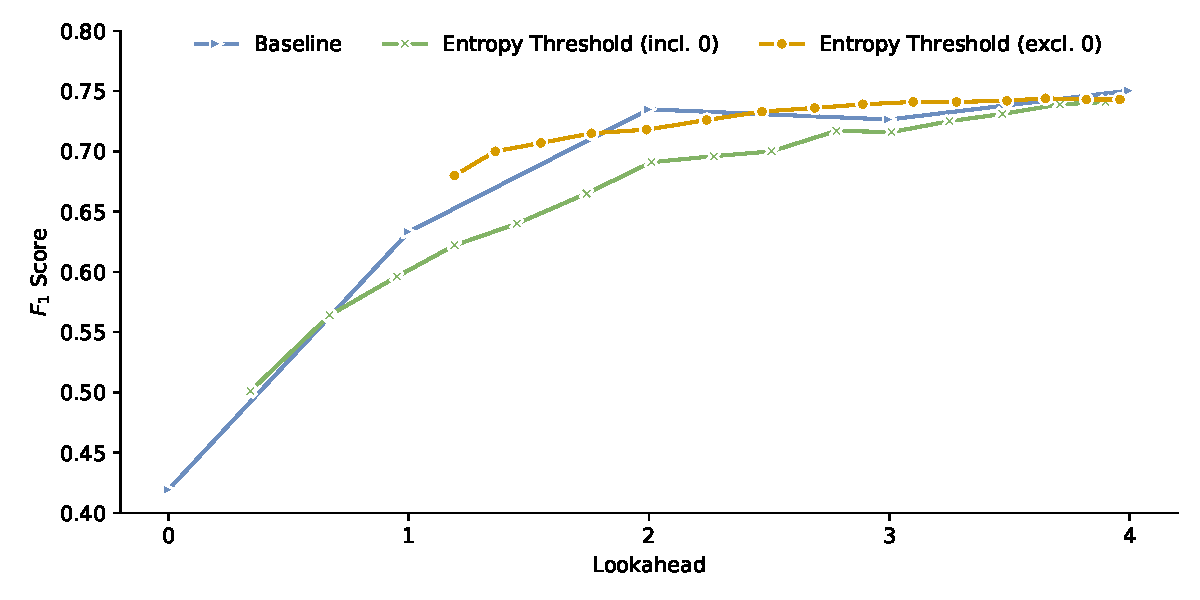
\includegraphics[width=.9\textwidth]{entropy.pdf}
\caption{The results of entropy threshold decoding.}
\label{fig:truncquant}
\end{figure}
\begin{table}[!htb]
\resizebox{\textwidth}{!}{%
\begin{tabular}{lcccccccccccc}
\hline
\multicolumn{1}{c}{\multirow{2}{*}{Train}} &
  \multicolumn{3}{c}{Full Stop} &
  \multicolumn{3}{c}{Comma} &
  \multicolumn{3}{c}{Question} &
  \multicolumn{3}{c}{Overall} \\ \cline{2-13} 
\multicolumn{1}{c}{} &
  \multicolumn{1}{r}{P} &
  R &
  \multicolumn{1}{c|}{$F_1$} &
  P &
  R &
  \multicolumn{1}{c|}{$F_1$} &
  P &
  R &
  \multicolumn{1}{c|}{$F_1$} &
  P &
  R &
  $F_1$ \\ \hline
\textit{$\text{IWSLT11}_{TRAIN}$ (Resampled)} &
  77.4 &
  87.6 &
  \multicolumn{1}{c|}{82.2} &
  55.0 &
  \textbf{87.1} &
  \multicolumn{1}{c|}{67.5} &
  {\ul 87.5} &
  {\ul 77.8} &
  \multicolumn{1}{c|}{{\ul 82.4}} &
  63.9 &
  \textbf{87.1} &
  73.7 \\
$+\text{IWSLT11}_{TRAIN,2\%}$ &
  76.4 &
  \textbf{89.9} &
  \multicolumn{1}{c|}{82.6} &
  64.0 &
  74.2 &
  \multicolumn{1}{c|}{68.7} &
  50.0 &
  80.0 &
  \multicolumn{1}{c|}{61.5} &
  70.4 &
  82.7 &
  76.0 \\
$+\text{IWSLT11}_{VALID,t_p=280ms}$ &
  \textbf{82.4} &
  88.1 &
  \multicolumn{1}{c|}{\textbf{85.1}} &
  63.0 &
  78.8 &
  \multicolumn{1}{c|}{70.0} &
  57.1 &
  80.0 &
  \multicolumn{1}{c|}{66.7} &
  {\ul 72.5} &
  {\ul 83.8} &
  {\ul 77.7} \\
$+\text{both}$ &
  {\ul 78.9} &
  {\ul 89.3} &
  \multicolumn{1}{c|}{{\ul 83.8}} &
  \textbf{67.8} &
  76.5 &
  \multicolumn{1}{c|}{\textbf{71.9}} &
  \textbf{88.1} &
  \textbf{78.3} &
  \multicolumn{1}{c|}{\textbf{82.9}} &
  \textbf{73.5} &
  83.4 &
  \textbf{78.2} \\ \hline
\textit{$\text{MGB}_{TRAIN}$ (Resampled)} &
  62.3 &
  \textbf{81.2} &
  \multicolumn{1}{c|}{{\ul 70.5}} &
  53.4 &
  \textbf{68.9} &
  \multicolumn{1}{c|}{\textbf{60.2}} &
  72.9 &
  \textbf{64.8} &
  \multicolumn{1}{c|}{\textbf{68.6}} &
  59.8 &
  \textbf{74.9} &
  {\ul 66.5} \\
$+\text{MGB}_{TRAIN,2\%}$ &
  \textbf{66.6} &
  {\ul 77.2} &
  \multicolumn{1}{c|}{\textbf{71.5}} &
  \textbf{63.9} &
  55.7 &
  \multicolumn{1}{c|}{59.5} &
  {\ul 73.3} &
  58.8 &
  \multicolumn{1}{c|}{65.2} &
  \textbf{66.2} &
  67.4 &
  \textbf{66.8} \\
$+\text{MGB}_{TRAIN,2\%,t_p=280ms}$ &
  64.8 &
  76.5 &
  \multicolumn{1}{c|}{70.2} &
  {\ul 61.0} &
  {\ul 58.3} &
  \multicolumn{1}{c|}{{\ul 59.6}} &
  \textbf{75.5} &
  62.1 &
  \multicolumn{1}{c|}{{\ul 68.1}} &
  {\ul 64.5} &
  {\ul 68.2} &
  66.3 \\
$+\text{both}$ &
  {\ul 65.4} &
  73.3 &
  \multicolumn{1}{c|}{69.2} &
  60.6 &
  56.9 &
  \multicolumn{1}{c|}{58.7} &
  70.2 &
  {\ul 62.7} &
  \multicolumn{1}{c|}{66.2} &
  64.2 &
  66.1 &
  65.2 \\ \hline
\end{tabular}%
}
\caption{Results of the \textsc{RoBERTa-large} model trained on a resampled training set.}
\label{tab:finalresults}
\end{table}
Recent state-of-the-art performance on the IWSLT11 dataset has been shown using the \textsc{base} and \textsc{large} variants of \textsc{RoBERTa}, which are twice and quadruple the size of the \textsc{DistilRoBERTa} model used thus far. \citet{li2020train} show evidence for large models outperforming small ones even when using the same computational time and resources. They show that larger models trained on smaller datasets outperform smaller models trained on large ones. To improve our model performance while restricting ourselves to a similar compute budget as for the \textsc{DistilRoBERTa} model, we use downsampling. We remove samples with no punctuation until there are twice the number of \texttt{None} samples than the number of samples for the most common punctuation mark. For the MGB dataset, this reduces the number of samples to 33\% of their original number. For the IWSLT11 dataset, the number of samples is reduced to 29\%. As this shifts the class priors, we also finetune on an unaltered subset of the data (2\% of the training data). Table \ref{tab:finalresults} shows these results in detail.
\subsubsection*{MGB}
We achieve results outperforming a previous RNN machine translation approach \citep{Klejch2016} while not using any language model data and only 33\% of the training data, pause features do not lead to any significant improvements. We reason that the general improvement can be attributed to the Transformer architecture, following the trend seen in other NLP domains \citep{transformersurvey}. \Ondrej{And also pretraining on large amounts of data}
\subsubsection*{IWSLT11}
Despite training on $29\%$ of the train dataset alone, we achieve an overall $F_1$-score of 78.2\% on the IWSLT11 test dataset, which, to the best of our knowledge, is the highest achieved without utilizing additional data from different domains such as POS-tags \citep{yi2020adversarial}, or disfluency data \citep{chen2020controllable,Lin2020disf} or using data augmentation \citep{sotapunctuation}.

\section{Inference Speed \& Quantization}
\begin{figure}[!htb]
\centering
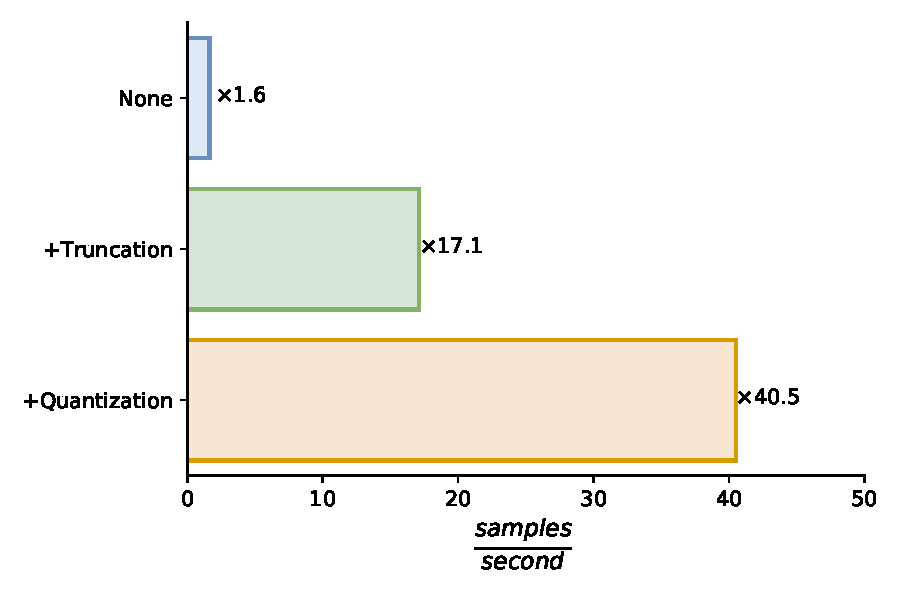
\includegraphics[width=.7\textwidth]{speedup.pdf}
\caption{Effect of truncation and quantization on inference speed.}
\label{fig:truncquant}
\end{figure}
We now evaluate inference speed of the final IWSLT11 model described above\footnote{A single core of a Ryzen 7 2700X processor was used, 6000 inference iterations were averaged.}. \Ondrej{I think that footnote should be after full stop.} While we observed a linear increase in speed while training (see section \ref{sec:trunc}), for inference, we get closer to the quadratic improvement expected. The theoretical upper bound for the speedup when using $\frac{1}{4}$ of the original window size is $\times16$. In our inference experiments, we find an actual increase in speed of $\times10.68$, from $1.6\frac{samples}{second}$ to $17.1\frac{samples}{second}$. To further increase model speed and decrease model size, we perform quantization of the model weights, reducing their size from \texttt{float32} to \texttt{int8}. We do this using standard procedures available in the PyTorch libary\footnote{\url{https://pytorch.org/tutorials/advanced/static_quantization_tutorial.html}} \citep{pytorch}. This leads to a slight decrease in model performance ($-1.3\%~F_1$ for MGB, $-2.6\%~F_1$ for IWSLT11). This also leads to a $\times2.36$ increase in speed to 40.5 $\frac{samples}{second}$ and $\approx\times4$ compression in model size, reducing model size from 1.4GB to 355MB. We reason that the decrease in performance observed could be offset by the compression and speed gained in certain use cases, for example for use on mobile devices.\Ondrej{Could be also improved by fine-tuning the quantized model}

\chapter{Conclusion and Future Work}

\section{Conclusions}
Rather than building a punctuation prediction system and then adapting it to the streamed ASR use case, we start with this streamed punctuation annotation use case in mind. Most recent punctuation annotation systems using Transformers use a sequence tagging approach. Contrary to this we use a classification approach and present a novel \emph{masked punctuation prediction} training and inference procedure inspired by the masked language modeling task \citep{devlin2019bert} used when pre-training Transformers. When performing streamed punctuation annotation, little right-side context is available. We show that the aforementioned tagging approach performs worse than our new method when a right-side context of 4 words or less is available. \\
To utilize acoustic information while relying on an ASR system's output alone, we encode timing information commonly provided by ASR systems as an additional feature. We achieve this by adding a special \texttt{[PAUSE]} token to the input. We show that while this token provides significant improvements on the IWSLT11 dataset, it does not lead to such improvements on the MGB dataset. We conclude that pause tokens are of limited use for the punctuation annotation of spontaneous speech, but can work well for datasets of a more scripted nature, and could be of great use for dictation systems.\\
We use downsampling to efficiently train our final model using $\approx\frac{1}{3}$ of the available training data, while achieving overall $F_1$ scores within 4.7\% (absolute) of the best model we are aware of on the IWSLT11 dataset \citep{sotapunctuation}. We also find that the advantages of the commonly used approach of fine-tuning pre-trained Transformer models extend to the semi-spontaneous speech present in the MGB dataset, as we are able to outperform the previous best model \citep{Klejch2016} by 2.9\% (absolute) on average for each evaluated punctuation mark. As we use a model pre-trained on an unsupervised language modeling task, we achieve this while utilizing 0.03\% of the data used to train the previous best model on the MGB dataset.\\
We show our classification approach can be combined with truncation, which leads to a $\times4$ speedup for training and $\times10$ speedup for inference while not decreasing performance. For use of ASR on low-resource devices, we show weight quantization yields a further $\times2.36$ speedup and a reduction in model size by $\times4$, while leading to a minor decrease in $F_1$ scores of 2\% on average.

\section{Future Work}
Future work could improve our system by adding teacher forcing, as a mechanism to use past punctuation predictions for future ones. Our naive Entropy Threshold Decoding algorithm could be replaced by a learned method, such as a shallow neural network to predict if more lookahead is needed. Quantization-aware training, in which floating point weights are regularly rounded during training, could help mitigate the loss in performance reported due to quantization.
While the improvement in inference speed gained using truncation are significant, we show that truncation starts to decrease model performance at a window width of 16 or less. This limits further improvements when reaching this window size. To further improve models for low-resource applications, efficient transformer architectures reducing the $\mathrm{O}(n^2)$ complexity of dot-product attention could be investigated. In our experiments on the IWSLT11 dataset, we show pause tokens at varying thresholds affect different punctuation mark performance. To allow the model to distinguish between pauses of different lengths, the pause features utilized in our work could be provided as an input to the final model head, or separate short- and long-pause tokens could be investigated. Finally, our system and the impact of \texttt{[PAUSE]} tokens could be evaluated on the ASR results, rather than transcriptions, of the MGB and IWSLT11 datasets.

\bibliography{bibfile_new}

%% You can include appendices like this:
\appendix
\addtocontents{toc}{\protect\setcounter{tocdepth}{-1}}
\chapter{Background}
 
\section{On Dataset Statistics in Table \ref{dspunc}}
\label{appendixds}
The train/evaluation/test splits for datasets used in punctuation annotation are inconsistent across papers, which means the percentages reported in \ref{dspunc} might vary from some of the evaluation sets used in punctuation papers. The sources for said numbers are as follows:
\begin{itemize}
    \item \citet{Ueffing2013} for WSJ and IWSLT11 corpus.
    \item \citet{kim2003} for BN corpus size and \citet{batista2008} for BN punctuation percentages.
    \item \citet{Klejch2016} for MGB corpus.
    \item \citet{europarl} for Europarl corpus.
\end{itemize}

Punctuation marks other than full stop, comma and question mark were reported for several corpora and are shown in the Table~below.
\\
\vspace{1cm}
\begin{adjustbox}{width=\columnwidth,center}
\begin{tabular}{|l|lllllll|}
\hline
\textbf{Dataset} & \textbf{Tokens} & \textbf{Full Stop} & \textbf{Comma} & \textbf{Question Mark} & \textbf{Exclamation Mark} & \textbf{Dash} & \textbf{Triple Dots} \\ \hline
WSJ              & 51,023          & 4.59\%             & 5.98\%         & 0.04\%                 & -                         & -             & -                    \\
IWSLT11              & 17,207          & 5.37\%             & 6.36\%         & 0.48\%                 & -                         & -             & -                    \\
MGB              & 92,622          & 7.63\%             & 4.77\%         & 1.67\%                 & 1.18\%                    & -             & 0.59\%               \\
BN               & 35,710          & 3.5\%              & 5.1\%          & 0.29\%                 & -                         & -             & -                    \\
Europarl         & 10,000          & 2.29\%             & 2.36\%         & 0.01\%                 & 0.01\%                    & 0.41\%        & -                    \\ \hline
\end{tabular}
\end{adjustbox}

\chapter{Experiments}
\section{On Truncation Window Sizes}

\begin{table}[h]
\resizebox{\textwidth}{!}{%
\begin{tabular}{@{}llcccc|ccc|ccc|ccc@{}}
\toprule
\multirow{2}{*}{Test} &
  \multicolumn{1}{c}{\multirow{2}{*}{Window}} &
  \multirow{2}{*}{$\cfrac{\text{samples}}{\text{second}}$} &
  \multicolumn{3}{c|}{Full Stop} &
  \multicolumn{3}{c|}{Comma} &
  \multicolumn{3}{c|}{Question} &
  \multicolumn{3}{c}{Overall} \\ \cmidrule(l){4-15} 
                         & \multicolumn{1}{c}{} &                     & P    & R    & $F_1$ & P    & R    & $F_1$ & P     & R    & $F_1$ & P    & R    & $F_1$ \\ \midrule
\multirow{5}{*}{IWSLT11} & $w=128$              & 572                 & 75.3 & 86.2 & 80.4  & 64.7 & 65.2 & 64.9  & 57.1  & 80.0 & 66.7  & 70.5 & 76.7 & 73.5  \\
                         & $w=64$               & 1258 ($\times2.19$) & 74.1 & 81.1 & 77.5  & 65.5 & 68.9 & 67.2  & 40.0  & 80.0 & 53.3  & 69.3 & 75.7 & 72.4  \\
                         & $w=32$               & 2340 ($\times1.86$) & 74.6 & 84.9 & 79.4  & 69.1 & 71.2 & 70.1  & 50.0  & 80.0 & 61.5  & 71.7 & 78.7 & 75.0  \\
                         & $w=16$               & 4724 ($\times2.01$) & 70.9 & 84.3 & 77.0  & 66.9 & 61.4 & 64.0  & 75.0  & 60.0 & 66.7  & 69.4 & 73.6 & 71.5  \\
                         & $w=8$                & 8060 ($\times1.70$) & 62.9 & 49.1 & 55.1  & 40.0 & 9.1  & 14.8  & 100.0 & 40.0 & 57.1  & 59.0 & 31.1 & 40.7  \\ \midrule
\multirow{5}{*}{MGB}     & $w=128$              & 581                 & 63.7 & 70.5 & 67.0  & 57.7 & 48.6 & 52.7  & 69.9  & 54.2 & 61.0  & 62.3 & 60.7 & 61.5  \\
                         & $w=64$               & 1241 ($\times2.13$) & 64.2 & 72.2 & 68.0  & 58.3 & 48.8 & 53.1  & 69.5  & 54.2 & 60.9  & 62.8 & 61.6 & 62.2  \\
                         & $w=32$               & 2387 ($\times1.92$) & 63.4 & 72.0 & 67.4  & 59.9 & 48.8 & 53.8  & 71.1  & 55.3 & 62.2  & 63.0 & 61.7 & 62.3  \\
                         & $w=16$               & 4649 ($\times1.94$) & 61.5 & 69.8 & 65.4  & 56.6 & 46.9 & 51.3  & 68.5  & 45.5 & 54.6  & 60.5 & 58.7 & 59.6  \\
                         & $w=8$                & 8004 ($\times1.72$) & 43.8 & 35.8 & 39.4  & 49.2 & 7.0  & 12.3  & 0.0   & 0.0  & 0.0   & 44.4 & 21.3 & 28.8  \\ \bottomrule
\end{tabular}%
}
\caption{Window size impacts on speed and performance.}
\label{tab:windowsize}
\end{table}

\end{document}
